%%%%%%%%%%%%%%%%%%%%%%%%%%%%%%%%%%%%%%%%%%%%%%%%%%%%%%%%%%%%%%%%%
% MUW Presentation
% LaTeX Template
% Version 1.0 (27/12/2016)
%
% License:
% CC BY-NC-SA 4.0 (http://creativecommons.org/licenses/by-nc-sa/3.0/)
%
% Created by:
% Nicolas Ballarini, CeMSIIS, Medical University of Vienna
% nicoballarini@gmail.com
% http://statistics.msi.meduniwien.ac.at/
%
% Customized for UAH by:
% David F. Barrero, Departamento de Automática, UAH
%%%%%%%%%%%%%%%%%%%%%%%%%%%%%%%%%%%%%%%%%%%%%%%%%%%%%%%%%%%%%%%%%

\documentclass[10pt,compress]{beamer} % Change 10pt to make fonts of a different size
\mode<presentation>

\usepackage[spanish]{babel}
\usepackage{fontspec}
\usepackage{tikz}
\usepackage{etoolbox}
\usepackage{xcolor}
\usepackage{xstring}
\usepackage{listings}
\usepackage{multicol}
\usepackage{tabularx}
\usepackage{tikz}
\usetikzlibrary{matrix,chains,positioning,decorations.pathreplacing,arrows,shapes}

\usetheme{UAH}
\usecolortheme{UAH}
\setbeamertemplate{navigation symbols}{} 
\setbeamertemplate{caption}[numbered]

%%%%%%%%%%%%%%%%%%%%%%%%%%%%%%%%%%%%%%%%%%%%%%%%%%%%%%%%%%%%%%%%%
%% Presentation Info
\title[Scientific Programming]{Scientific Programming in Python}
\author{\asignatura\\\carrera}
\institute{}
\date{Departamento de Automática}
%%%%%%%%%%%%%%%%%%%%%%%%%%%%%%%%%%%%%%%%%%%%%%%%%%%%%%%%%%%%%%%%%


%%%%%%%%%%%%%%%%%%%%%%%%%%%%%%%%%%%%%%%%%%%%%%%%%%%%%%%%%%%%%%%%%
%% Descomentar para habilitar barra de navegación superior
\setNavigation
%%%%%%%%%%%%%%%%%%%%%%%%%%%%%%%%%%%%%%%%%%%%%%%%%%%%%%%%%%%%%%%%%

%%%%%%%%%%%%%%%%%%%%%%%%%%%%%%%%%%%%%%%%%%%%%%%%%%%%%%%%%%%%%%%%%
%% Configuración de logotipos en portada
%% Opacidad de los logotipos
\newcommand{\opacidad}{1}
%% Descomentar para habilitar logotipo en pié de página de portada
\renewcommand{\logoUno}{Images/isg.png}
%% Descomentar para habilitar logotipo en pié de página de portada
%\renewcommand{\logoDos}{Images/CCLogo.png}
%% Descomentar para habilitar logotipo en pié de página de portada
%\renewcommand{\logoTres}{Images/ALogo.png}
%% Descomentar para habilitar logotipo en pié de página de portada
%\renewcommand{\logoCuatro}{Images/ELogo.png}
%%%%%%%%%%%%%%%%%%%%%%%%%%%%%%%%%%%%%%%%%%%%%%%%%%%%%%%%%%%%%%%%%

%%%%%%%%%%%%%%%%%%%%%%%%%%%%%%%%%%%%%%%%%%%%%%%%%%%%%%%%%%%%%%%%%
%% FOOTLINE
%% Comment/Uncomment the following blocks to modify the footline
%% content in the body slides. 


%% Option A: Title and institute
\footlineA
%% Option B: Author and institute
%\footlineB
%% Option C: Title, Author and institute
%\footlineC
%%%%%%%%%%%%%%%%%%%%%%%%%%%%%%%%%%%%%%%%%%%%%%%%%%%%%%%%%%%%%%%%%

\begin{document}

%%%%%%%%%%%%%%%%%%%%%%%%%%%%%%%%%%%%%%%%%%%%%%%%%%%%%%%%%%%%%%%%%
% Use this block for a blue title slide with modified footline
{\titlepageBlue
    \begin{frame}
        \titlepage
    \end{frame}
}

\institute{\asignatura}

\begin{frame}[plain]{}
	\begin{block}{Objectives}
		\begin{enumerate}
		\item Introduce some Python tools for scientific programming.
		\item Motivate the need of efficient matrix manipulation.
		\item Handle matrices and dataframes in Python.
		\item Basic data visualization with Python.
		\end{enumerate}
	\end{block}

   \begin{block}{Bibliography}
       Jake VanderPlas. \textit{Python Data Science Handbook}. Chapters 1, 2, 3 and 4. O'Reilly. \href{https://jakevdp.github.io/PythonDataScienceHandbook/}{(Link)}.
   \end{block}

\end{frame}

{
\disableNavigation{white}
\begin{frame}[shrink]{Table of Contents}
 \frametitle{Table of Contents}
 \begin{multicols}{2}
 \tableofcontents
 \end{multicols}
  % You might wish to add the option [pausesections]
\end{frame}
}

\section{Overview}

\subsection{Data Science}

\begin{frame}{Overview}{Data Science}
	\begin{figure}
		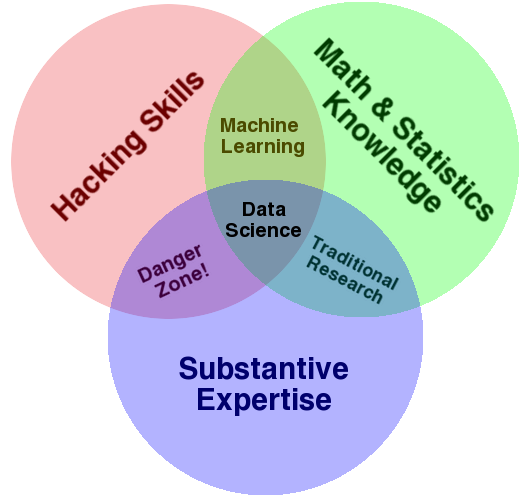
\includegraphics[scale=0.35]{figs/Data_Science_VD.png}	
	\end{figure}				
\end{frame}

\subsection{The data scientist toolkit}

\begin{frame}{Data Science}{The data scientist tookit (I)}
	Data science is about manipulating data
	\begin{itemize}
		\item Need of specialized tools
		\item Two main languajes: R and Python
	\end{itemize}
	Python is a general purpose programming language
	\begin{itemize}
		\item Easy integration 
		\item Huge ecosystem of packages and tools
	\end{itemize}
	Need of data-oriented tools
	\begin{itemize}
		\item Features provided by third-party tools
	\end{itemize}

\end{frame}

\begin{frame}{Data Science}{The data scientist tookit (II)}
   \begin{tabular}{cll}\hline
       \textbf{Tool}& \textbf{Type} & \textbf{Description}\\ \hline
	   \texttt{iPython} & Software & Advaced Python interpreter \\
	   \texttt{Jupiter} & Software & Python notebooks (Python interpreter) \\
	   \texttt{Numpy}   & Package  & Efficient array operations \\
	   \texttt{Pandas}  & Package  & Dataframe support \\
	   \texttt{Matplotlib} & Package & Data visualization \\
	   \texttt{Seaborn} & Package & Data visualization with dataframes \\
	   \texttt{Scikit-learn} & Package & AI/ML package for Python \\
	   \hline
   \end{tabular}
\end{frame}

\subsection{Anaconda}
\begin{frame}{Data Science}{Anaconda}
    \begin{columns}
 	   \column{.6\textwidth}
   All those tools are packaged in \texttt{Anaconda}
   \begin{itemize}
   		\item Python distribution for Data Science
	\end{itemize}

	Anaconda provides \texttt{Spyder}
	\begin{itemize}
		\item Python IDE designed for Data Science
	\end{itemize}

	Other tools provided by Anaconda
	\begin{itemize}
		\item Conda: Packages management tool
		\item TensorFlow: Deep Learning 
		\item Many others
	\end{itemize}

 		\column{.4\textwidth}
			
\includegraphics[width=0.6\textwidth]{figs/Anaconda_Logo.png} \\\bigskip
			
\includegraphics[width=0.6\textwidth]{figs/spyder.png}	
			%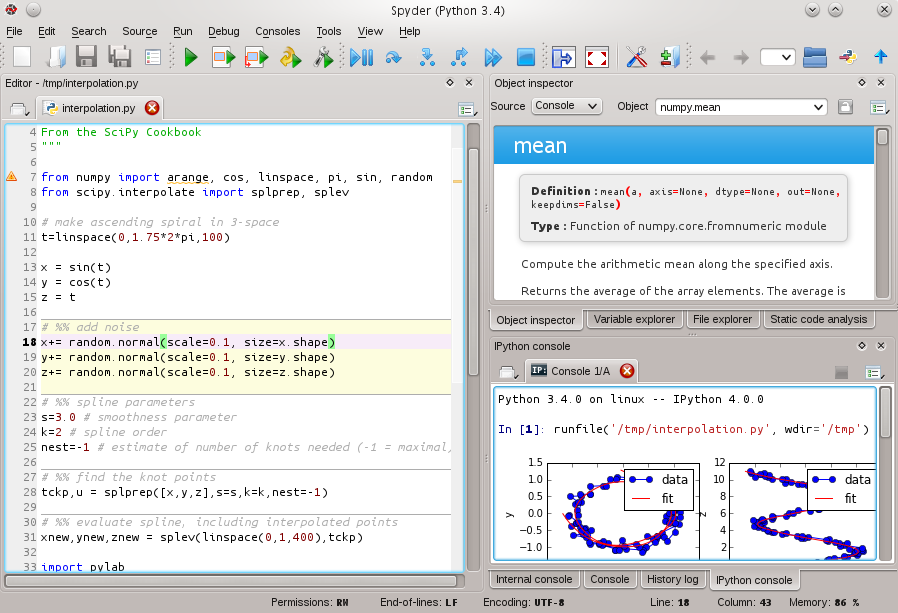
\includegraphics[width=0.6\textwidth]{figs/spyder-ide.png}	
	\end{columns}
\end{frame}

\subsection{Python IDEs for Data Science}
\begin{frame}{Data Science}{Python IDEs for Data Science (I)}
    \begin{columns}[t]
 	   \column{.25\textwidth}
	   \centering \textbf{iPython}\\
	   iPython = Interactive Python
   		\begin{itemize}
		\item Extended funcionality
		\item Enhanced UI
		\item External editor
		\end{itemize}

		Running iPython:\\
		\texttt{\$ ipython}

 	   \column{.25\textwidth}
	   \centering \textbf{Jupyter}\\
		Python notebooks
	\begin{itemize}
		\item Web-based IDE
		\item Documentation
		\item Integration with GitHub
		\item Uses iPython
	\end{itemize}

		Running Jupyter:\\
		\texttt{\$ jupyter notebook}

		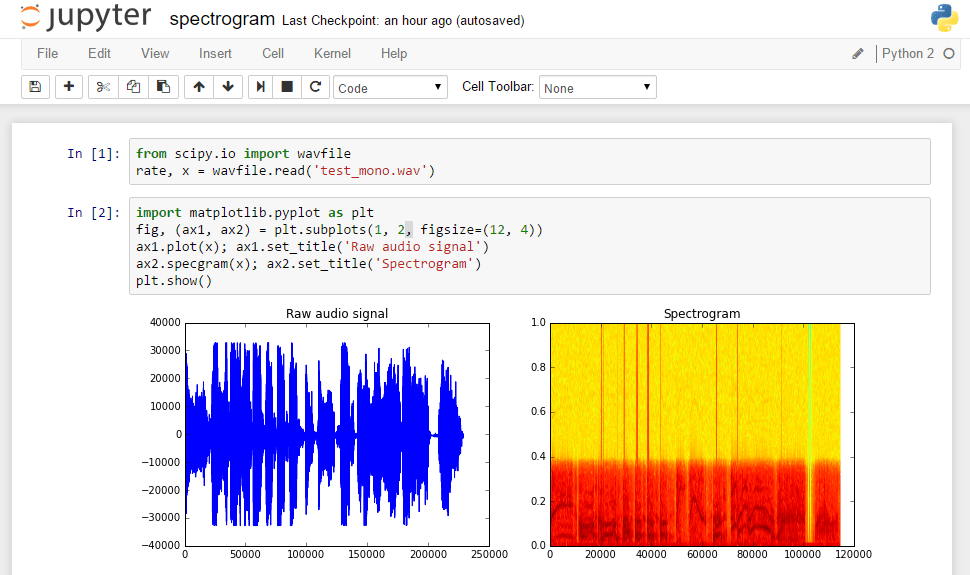
\includegraphics[width=0.8\textwidth]{figs/jupyter.png}	

 	\column{.25\textwidth}
	   \centering \textbf{Rodeo}\\
		Python version of RStudio
		\begin{itemize}
			\item Good for R developers
			\item Not included in Anaconda
			\item Uses iPython
		\end{itemize}
        
        \bigskip

		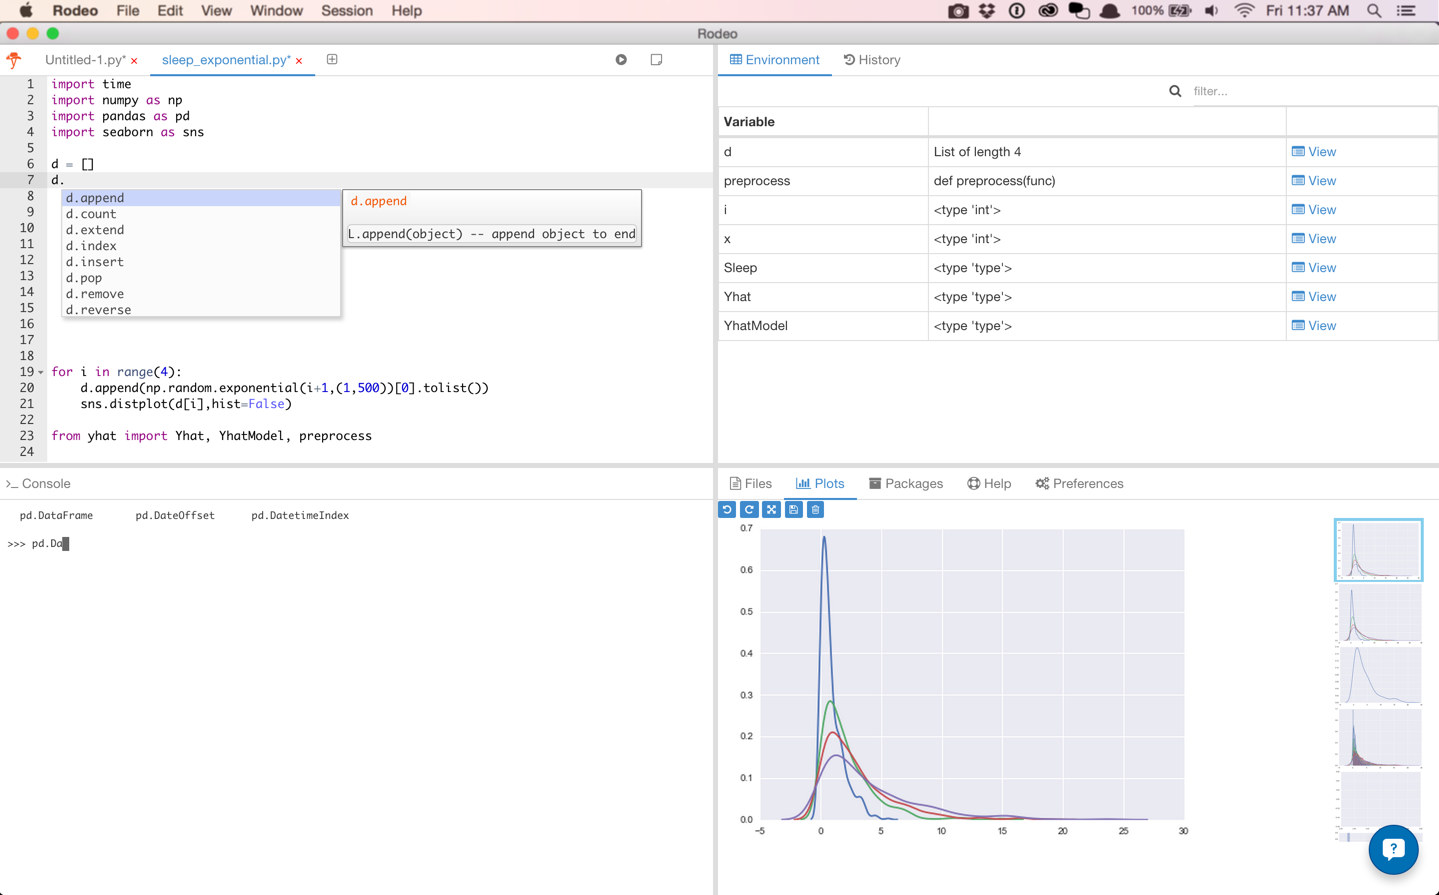
\includegraphics[width=0.8\textwidth]{figs/rodeo.png}	

 	\column{.25\textwidth}
	   \centering \textbf{Spyder}\\
		Matlab-like IDE

        \bigskip

		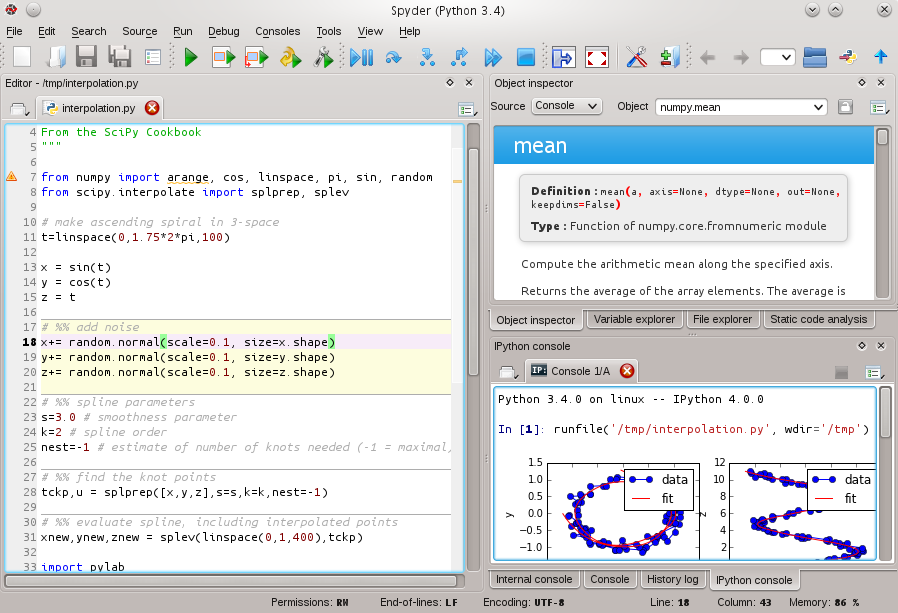
\includegraphics[width=0.8\textwidth]{figs/spyder-ide.png}	

	\end{columns}
\end{frame}

\begin{frame}{Data Science}{Python IDEs for Data Science (II)}
    \begin{block}{Exercises}
		Write a Python script that shows the multiplication table of the number 5. Write the script using each one of the following environments:
   		\begin{enumerate}
   		\item iPython + text editor of your choice.
		\item Jupiter. 
            \begin{itemize}
                \item Bonus track: Publish the notebook in GitHub.
            \end{itemize}
		\item Spyder.
		\item Rodeo.
		\end{enumerate}
	\end{block}
\end{frame}

\section{Basics}
\begin{frame}{iPython}{Basics (I)}
    In regular Python ...
    \begin{itemize}
        \item most objects come with a docstring attribute
        \item docstring accesible thorugh \texttt{help()}
    \end{itemize}
    iPython provides `\texttt{?}', a shortcut to \texttt{help()}
    \begin{itemize}
        \item \texttt{len?}, \texttt{list?}, \texttt{list.append?}
        \item Try to type just `\texttt{?}'
    \end{itemize}
    Easy access to source code with `\texttt{??}'
    \begin{itemize}
        \item Does not work with most buildin functions!
    \end{itemize}
\end{frame}

\begin{frame}{iPython}{Basics (II)}
    Press \texttt{<tab>} to complete almost everything
    \begin{itemize}
        \item Object contents\\
	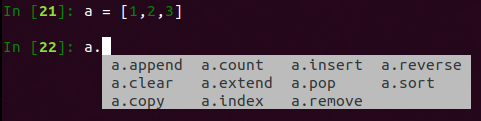
\includegraphics[width=0.45\textwidth]{figs/tab.png} 
        \item Packages\\
	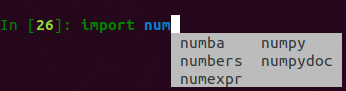
\includegraphics[width=0.36\textwidth]{figs/tab2.png}	
        \item Wildcards\\
	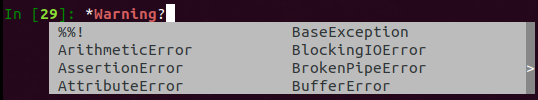
\includegraphics[width=0.45\textwidth]{figs/tab3.png}	
    \end{itemize}
\end{frame}

\begin{frame}{iPython}{Basics (III): Keyboard shortcuts}
    \footnotesize{
        Navigation\\
        \begin{tabular}{ll}\hline
       \textsc{Keystroke} &  \textsc{Action}\\ \hline
	   \texttt{Ctrl-a} & Move cursor to the beginning of the line  \\
	   \texttt{Ctrl-e} & Move cursor to the end of the line  \\
	   \texttt{Ctrl-b} & Move cursor back one character  \\
	   \texttt{Ctrl-f} & Move cursor forward one character  \\\hline
        \end{tabular}

    \bigskip
     History\\
       \begin{tabular}{ll}\hline
       \textsc{Keystroke} &  \textsc{Action}\\ \hline
       \texttt{Ctrl-p ($\uparrow$)} & Previous command  \\
       \texttt{Ctrl-n ($\downarrow$)} & Next command  \\
	   \texttt{Ctrl-r} & Reverse-search  \\\hline
    \end{tabular}

    \bigskip
        Text entry\\
        \begin{tabular}{ll}\hline
       \textsc{Keystroke} &  \textsc{Action}\\ \hline
	   \texttt{Ctrl-d} & Delete next character in line  \\
	   \texttt{Ctrl-k} & Cut text from cursor to end of line  \\
	   \texttt{Ctrl-u} & Cut text from beginning of line to cursor  \\
       \texttt{Ctrl-y} & Yank (paste) previously cut text  \\\hline
       \end{tabular}
   }
\end{frame}

\subsection{Magic commands}
\begin{frame}{iPython}{iPython magic commands}
	Magic commands: iPython extension of Python syntax
	\begin{itemize}
	\item Not valid in regular Python
	\item Provides handly features
	\item Widely used in DS and ML
	\end{itemize}
	Two flavours
	\begin{itemize}
	\item \% prefix: Line magics - single line
	\item \%\% prefix: Cell magics - several lines
	\end{itemize}
	Help available
	\begin{itemize}
		\item \texttt{\%magic}: Magic commands
		\item \texttt{\%lsmagic}: List of magic commands
	\end{itemize}
\end{frame}

\subsection{Pasting code blocks}
\begin{frame}[fragile]{iPython}{Pasting code blocks: \texttt{\%paste} and \texttt{\%cpaste}}
    \begin{columns}
 	   \column{.5\textwidth}
	   Pasting code in Python is troublesome
		\begin{itemize}
			\item \texttt{\%paste}: Paste one time
			\item \texttt{\%\%cpaste}: Paste several times
		\end{itemize}
 	   \column{.5\textwidth}
	       %\begin{block}{}
		   %    \vspace{-0.2cm}
		   %    \lstinputlisting{code/donothing.py}
		   %    \vspace{-0.2cm}
		   %\end{block}
	   \begin{exampleblock}{}
	   \vspace{-0.2cm}
		\begin{lstlisting}
def donothing(x):
    return x
		\end{lstlisting}
	   \vspace{-0.2cm}
	   \end{exampleblock}

	   \vspace{-0.2cm}
	\end{columns}

	\footnotesize{
    \begin{columns}
 	   \column{.4\textwidth}
		 \begin{exampleblock}{\footnotesize{\%paste}}
	   \vspace{-0.2cm}
	   \begin{verbatim}
In [20]: %paste
   def donothing(x):
 	  return x

## -- End pasted text --
\end{verbatim}
	   \vspace{-0.2cm}
	   \end{exampleblock}

	   \vspace{-0.2cm}

 	   \column{.6\textwidth}

	 	\begin{exampleblock}{\footnotesize{\%cpaste}}
	   \vspace{-0.2cm}
	   \begin{verbatim}
In [25]: %cpaste
Pasting code; enter '--' alone on the line
to stop or use Ctrl-D.
:       def donothing(x):
            return x:
:--
	   \end{verbatim}
	   \vspace{-0.2cm}
	   \end{exampleblock}
	   \end{columns}
	   }
\end{frame}

\subsection{Running external code}
\begin{frame}[fragile]{iPython}{Running external code: \texttt{\%run} and \texttt{\%timeit}}
    \begin{columns}
 	   \column{.4\textwidth}
	   \texttt{\%run}: Execute script
		\begin{itemize}
			\item Many optional arguments
			\item Checkout \texttt{\%run?}
		\end{itemize}
		\footnotesize{
	   \begin{exampleblock}{}
	   \vspace{-0.2cm}
	   \begin{verbatim}
In [40]: %run donothing.py

In [41]: donothing(10)
Out[41]: 10
	   \end{verbatim}
	   \vspace{-0.2cm}
	   \end{exampleblock}
		}

 	   \column{.6\textwidth}
	   \texttt{\%timeit}: Computes execution time
		\begin{itemize}
			\item Executes a single line
			\item Automatic adjustment of runs
			\item Shows basic statistics
		\end{itemize}

		\footnotesize{
	   \begin{exampleblock}{}
	   \vspace{-0.2cm}
	   \begin{verbatim}
In [33]: %timeit [n ** 2 for n in range(200)]
71.6 µs ± 1.84 µs per loop 
(mean ± std. dev. of 7 runs, 10000 loops each)

In [34]: %timeit [n ** 2 for n in range(2000)]
753 µs ± 16.2 µs per loop 
(mean ± std. dev. of 7 runs, 1000 loops each)
\end{verbatim}
	   \vspace{-0.2cm}
	   \end{exampleblock}
		}

		\normalsize{
	   \texttt{\%\%timeit}: Several lines\\
	   }
	\end{columns}

\end{frame}

\subsection{Input and output history}
\begin{frame}[fragile]{iPython}{Input and output history (I)}
	\begin{columns}
 	   \column{.6\textwidth}
	iPython stores its history as objects
	\begin{itemize}
		\item \texttt{In}: Input commands
			\begin{itemize}
			\item List storing commands
			\end{itemize}
		\item \texttt{Out}: Commands output
			\begin{itemize}
			\item Dictionary storing outputs
			\item Not all commands have outputs
			\end{itemize}
	\end{itemize}

	\vspace{-0.2cm}

 	   \column{.4\textwidth}
	\begin{exampleblock}{}
In [1]: import math

In [2]: math.sin(2)

Out[2]: 0.9092974268256817

In [3]: math.cos(2)

Out[3]: -0.4161468365471424

In [4]: Out[2] ** 2 + Out[3] ** 2

Out[4]: 1.0
	\end{exampleblock}
	\end{columns}
\end{frame}

\begin{frame}{iPython}{Input and output history (II)}
	Fast access to history: Underscore (\_)
	\begin{itemize}
		\item Variable containing the last output
		\item Example: \texttt{print(\_)}
	\end{itemize}
	Double and triple underscores
	\begin{itemize}
		\item Example: \texttt{print(\_\_)}
		\item Example: \texttt{print(\_\_\_)}
	\end{itemize}
	Trick: Shortcut to access ($\_n$)
	\begin{itemize}
		\item Out[n] = \_n, with n=number
		\item Example: \texttt{print(\_2)}
	\end{itemize}
	Magic command to show history
		\begin{itemize}
		\item \texttt{\%history}
		\end{itemize}
	Supressing command output (\texttt{;})
		\begin{itemize}
		\item Example: \texttt{4 * 2;}
		\end{itemize}
\end{frame}

\subsection{iPython shell commands}
\begin{frame}{iPython}{iPython shell commands}
	iPython provides easy interaction with the shell
	\begin{itemize}
		\item Execution of shell commands from iPython
		\item Use prefix `\texttt{!}'
		\item Example: \texttt{!ls}, \texttt{!pwd}
	\end{itemize}
	Save shell output in Python variables
	\begin{itemize}
		\item Example: \texttt{files = !ls}
	\end{itemize}
	Use Python variables in shell
	\begin{itemize}
		\item Example: \texttt{!echo \{files\}}
	\end{itemize}
\end{frame}

\subsection{Automagic}

\begin{frame}[fragile]{iPython}{Automagic}
	\begin{columns}
 	   \column{.4\textwidth}
	Problems with some shell commands
	\begin{exampleblock}{}
In [23]: !pwd

/repositorios/pythonCourse


In [24]: !cd ..


In [25]: !pwd

/repositorios/pythonCourse
	\end{exampleblock}
	Some magic commands here to help
	\begin{itemize}
		\item \texttt{\%cd}, \texttt{\%ls}, \texttt{\%mkdir}, \texttt{\%pwd}, ...
	\end{itemize}

 	   \column{.4\textwidth}
	Those magics are regularly used ...
	\begin{itemize}
		\item ... so common that \% is no longer required (automagic)
		\item Working with iPython is almost like working with a Unix-like shell
	\end{itemize}
	\footnotesize{
	\begin{block}{\footnotesize{Automagic commands}}
\texttt{cat}, \texttt{cp}, \texttt{env}, \texttt{ls}, \texttt{man}, \texttt{mkdir}, \texttt{more}, \texttt{mb}, \texttt{pwd}, \texttt{rm} and \texttt{rmdir}
	\end{block}
	}
	\end{columns}

\end{frame}

\section{NumPy}
\subsection{Understanding Data Types in Python}

\begin{frame}{NumPy}{Understanding Data Types in Python (I)}
    %Python supports matrices by default
    %\begin{itemize}
    %    \item Why do we need additional support?
	%\end{itemize}

    \begin{columns}
 	   \column{0.5\textwidth}
			
			\begin{block}{\footnotesize{Static typing}}
			\vspace{-0.2cm} 
				\lstinputlisting[basicstyle=\ttfamily\scriptsize,language=C]{code/static.c}
			\vspace{-0.2cm} 
			\end{block}

			\begin{itemize}
				\item Data types must be declared
				\item Data types cannot change
				\item Error detection in compilation
				\item Variables names are, basicly, labels
			\end{itemize}
			
 	   \column{0.5\textwidth}
			\begin{block}{\footnotesize{Dynamic typing}}
			\vspace{-0.2cm} 
				\lstinputlisting[basicstyle=\ttfamily\scriptsize]{code/dynamic.py}
			\vspace{-0.2cm} 
			\end{block}

			\begin{itemize}
				\item Data types are not declared
				\item Data types can change
				\item Error detection in run-time
				\item Variables are complex data structures (even for simple types)
			\end{itemize}
	\end{columns}
\end{frame}

\begin{frame}{NumPy}{Understanding Data Types in Python (II)}
    %Python supports matrices by default
    %\begin{itemize}
    %    \item Why do we need additional support?
	%\end{itemize}

	Dynamic typing must be implemented somewhere ...

    \begin{columns}
 	   \column{0.5\textwidth}
			\begin{block}{\footnotesize{Python 3.4 source code}}
			\vspace{-0.2cm} 
				\lstinputlisting[basicstyle=\ttfamily\scriptsize, language=C]{code/long.c}
			\vspace{-0.2cm} 
			\end{block}

 	   \column{0.5\textwidth}
			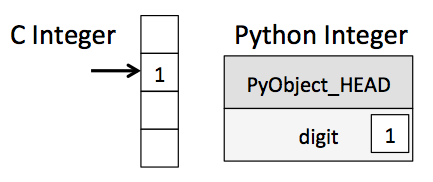
\includegraphics[width=\textwidth]{figs/cint_vs_pyint.png}	
	\end{columns}

\end{frame}

\begin{frame}[fragile]{NumPy}{Understanding Data Types in Python (III)}
	\begin{columns}
 	   \column{0.5\textwidth}
			A Python list may contain different types

 	   \column{0.5\textwidth}
	   \begin{exampleblock}{}
			\vspace{-0.2cm} 
			\lstinputlisting[basicstyle=\ttfamily\scriptsize]{code/lists.txt}
			\vspace{-0.2cm} 
		\end{exampleblock}
	\end{columns}

	\bigskip

	\centering 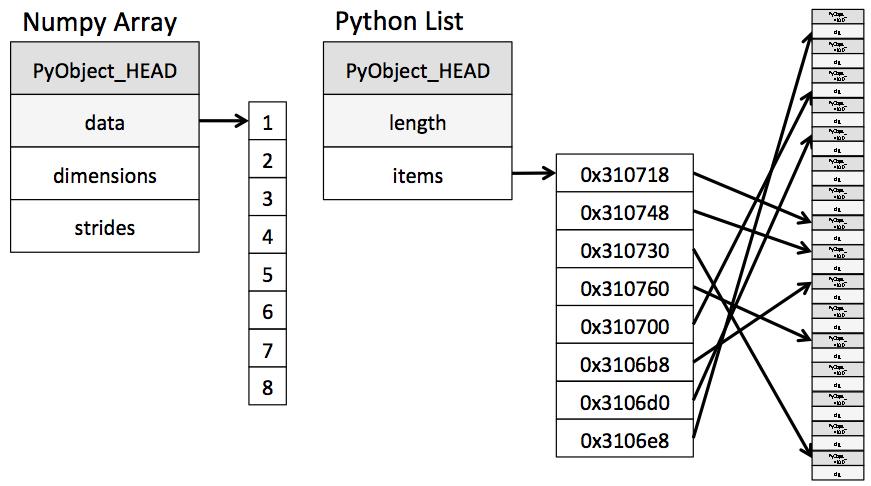
\includegraphics[width=0.8\textwidth]{figs/array_vs_list.png}	
\end{frame}

\begin{frame}[fragile]{NumPy}{Understanding Data Types in Python (IV)}
	Standard Python data types are powerful and flexible
	\begin{itemize}
		\item Flexibility has a price: Reduced performance
		\item Not an big issue in generic programming
		\item A big issue in scientific programming
		\item We require efficient data manipulation mechanisms: NumPy
	\end{itemize}
	NumPy: Python package for numeric computation
	\begin{itemize}
		\item Efficient array implementation
		\item Fast mathematical functions
		\item Random numbers generation
		\item Static data types: Less flexibility
	\end{itemize}
	Most Python modules for AI/ML depend on NumPy, in particular
	\begin{itemize}
		\item Pandas (dataframes), Scikit-learn (ML), Seaborn (data visualization)
	\end{itemize}
\end{frame}

\subsection{Introduction}
\begin{frame}[fragile]{NumPy}{Introduction}
	\begin{columns}
 	   \column{0.6\textwidth}
		NumPy must be imported in order to be available
		\begin{itemize}
			%\item By convention, \texttt{import numpy as np}
			\item Remember, you can use \texttt{np?} or \texttt{np.<TAB>}
		\end{itemize}

		The main component of NumPy is \alert{ndarray}
		\begin{itemize}
			\item Python object
			\item Efficient matrix representation
			\item Homogeneus elements
		\end{itemize}

 	   \column{0.4\textwidth}
		\begin{block}{\footnotesize{Convention}}
		\vspace{-0.2cm} 
			\begin{lstlisting}
			import numpy as np
			\end{lstlisting}
		\vspace{-0.2cm} 
		\end{block}

		\begin{exampleblock}{}
		\vspace{-0.2cm} 
			\begin{lstlisting}
			In [1]: array = np.array([1,2,3])
			In [2]: array
			Out[1]: array([1, 2, 3])
			In [3]: array = np.array([[1,2],[3,4]])
			\end{lstlisting}
		\vspace{-0.2cm} 
		\end{exampleblock}
	\end{columns}

\end{frame}

\subsection{Matrix creation}
\begin{frame}[fragile]{NumPy}{Matrix creation}
	NumPy functions for array creation from lists
	\begin{itemize}
		\item Lists must contain the same type, NumPy will upcast if needed
		\item \texttt{np.array([1, 4, 2, 5, 3])}
		\item \texttt{np.array([1, 2, 3, 4], dtype='float32')}: Explicit data type
		\item \texttt{np.array([3.14, 4, 2, 3])}: Upcast
	\end{itemize}
	NumPy functions for array creation from scratch
	\begin{itemize}
		\item \texttt{np.zeros(10, dtype=int)}: All zeros
		\item \texttt{np.ones((3, 5), dtype=float)}: All ones
		\item \texttt{np.full((3, 5), 3.14)}: Fill matrix
		\item \texttt{np.arange(0, 20, 2)}: Similar to Python's range()
		\item \texttt{np.linspace(0, 1, 5)}: Evenly spaced numbers
		\item \texttt{np.random.random((3, 3))}: Random numbers
		\item \texttt{np.random.normal(0, 1, (3, 3))}: Random normal numbers
		\item \texttt{np.random.randint(0, 10, (3, 3))}: Random integers
		\item \texttt{np.eye(3)}: Identity matrix
		\item \texttt{np.empty(3)}: Empty matrix
	\end{itemize}
\end{frame}

\subsection{NumPy data types}
\begin{frame}[fragile]{NumPy}{NumPy data types}
	\begin{columns}
 	   \column{0.4\textwidth}
	   Python is implemented in C
	   \begin{itemize}
	   	\item Data types in NumPy are based on those in C
	   \end{itemize}
	   Two styles to declare types
	   \begin{itemize}
	   	\item String:\\ \texttt{np.zeros(10, dtype='int16')}
		\item NumPy object: \texttt{np.zeros(10, dtype=np.int16)}
	   \end{itemize}

 	   \column{0.6\textwidth}
	\footnotesize{
    \begin{tabular}{ll}\hline
       \textsc{Data type} &  \textsc{Description}\\ \hline
	   \texttt{bool\_} & Boolean (True or False) stored as a byte  \\
	   \texttt{int\_} & Default integer type  \\
	   \texttt{intc} & Identical to C  \\
	   \texttt{intp} & Integer used for indexing  \\
	   \texttt{int8} & Byte  \\
	   \texttt{int16} & Integer  \\
	   \texttt{int32} & Integer  \\
	   \texttt{int64} & Integer  \\
	   \texttt{uint8} & Unsigned integer  \\
	   \texttt{uint16} & Unsigned integer  \\
	   \texttt{uint32} & Unsigned integer  \\
	   \texttt{uint64} & Unsigned integer  \\
	   \texttt{float\_} & Shorthand for float64  \\
	   \texttt{float16} & Half precision float  \\
	   \texttt{float32} & Single precision float  \\
	   \texttt{float64} & Double precision float  \\
	   \texttt{complex\_} & Shorthand for complex128  \\
	   \texttt{complex64} & Complex number  \\
	   \texttt{complex128} & Complex number  \\\hline
    \end{tabular}
	}
	\end{columns}
\end{frame}

\subsection{NumPy array attributes}
\begin{frame}[fragile]{NumPy}{NumPy array attributes}
	\begin{columns}
 	   \column{0.5\textwidth}
		Ndarray objects expose several attributes
		\begin{itemize}
			\item \texttt{ndim}: Dimensions
			\item \texttt{shape}: Size of each dimension
			\item \texttt{size}: Number of elements
			\item \texttt{dtype}: Data type
			\item \texttt{itemsize}: Size of each element (in bytes)
			\item \texttt{nbytes}: Size of the array (in bytes)
		\end{itemize}

 	   \column{0.5\textwidth}
		\begin{exampleblock}{}
		\vspace{-0.2cm} 
			\begin{lstlisting}
x = np.random.randint(10, size=(3, 4))
print("x3 ndim: ", x3.ndim)
print("x3 shape:", x3.shape)
print("x3 size: ", x3.size)
print("dtype:", x3.dtype)
print("itemsize:", x3.itemsize)
print("nbytes:", x3.nbytes)
			\end{lstlisting}
		\vspace{-0.2cm} 
		\end{exampleblock}
	\end{columns}
\end{frame}

\subsection{Accessing single elements}
\begin{frame}[fragile]{NumPy}{Accessing single elements}
	\begin{columns}
 	   \column{0.5\textwidth}
		Unidimensional array
		\begin{itemize}
			\item \texttt{array[index]}
		\end{itemize}
		Unidimensional array from the end
		\begin{itemize}
			\item \texttt{array[-index]}
		\end{itemize}
		Multidimensional array
		\begin{itemize}
			\item \texttt{array[row,column]}
		\end{itemize}

 	   \column{0.5\textwidth}
		\begin{exampleblock}{}
		\vspace{-0.2cm} 
			\begin{lstlisting}
x = np.array([5, 0, 3, 3, 7, 9])
x[0] # 5
x[4] # 7
x[-1] # 9
x[-2] # 7
x = np.array([[3, 5, 2, 4],
    [7, 6, 8, 8],
    [1, 6, 7, 7]])
x2[2, 0] # 1 
x2[2, -1] # 7
			\end{lstlisting}
		\vspace{-0.2cm} 
		\end{exampleblock}
	\end{columns}

	\smallskip

	\begin{columns}
 	   \column{0.6\textwidth}
		\begin{alertblock}{Warning}
			Ndarray has fixed types, values can be truncaded without warning. Big source of problems!
		\end{alertblock}
	\end{columns}

\end{frame}

\subsection{Accessing subarrays}
\begin{frame}[fragile]{NumPy}{Accessing subarrays}
	\begin{columns}
 	   \column{0.5\textwidth}
		Slice notation can be used with ndarray
		\begin{itemize}
			\item \texttt{x[start:stop:step]}
		\end{itemize}
		Default values
		\begin{itemize}
			\item Start = 0
			\item Stop = Size of dimension
			\item Step = 1
		\end{itemize}
		Step may take a negative value
		\begin{itemize}
			\item Reverse order
		\end{itemize}
		These operations return a view 
		\begin{itemize}
			\item Use \texttt{copy()} to get a copy
		\end{itemize}

 	   \column{0.5\textwidth}
		\begin{exampleblock}{\footnotesize{Unidimensional array}}
		\vspace{-0.2cm} 
			\begin{lstlisting}
x[:5]   # first five elements
x[5:]   # elements after index 5
x[4:7]  # middle sub-array
x[::2]  # every other element
x[1::2] # every other element, starting at index 1
x[::-1] # all elements, reversed
			\end{lstlisting}
		\vspace{-0.2cm} 
		\end{exampleblock}

		\begin{exampleblock}{\footnotesize{Multidimensional a  rray}}
		\vspace{-0.2cm} 
			\begin{lstlisting}
x[:2, :3]  # 2 rows, 3 columns
x[:3, ::2] # all rows, every other column
x[::-1, ::-1]
			\end{lstlisting}
		\vspace{-0.2cm} 
		\end{exampleblock}
	\end{columns}
\end{frame}

\subsection{Reshaping of arrays}
\begin{frame}[fragile]{NumPy}{Reshaping of arrays}
	\begin{columns}
 	   \column{0.5\textwidth}
		Reshaping arrays is a very common task
		\begin{itemize}
			\item Change data number of dimensions
			% Ejemplo imagen en red neuronal
		\end{itemize}
		Important ndarray method: \texttt{reshape()}
		\begin{itemize}
			\item Changes the dimensions of an array
			\item Sizes must match
		\end{itemize}

 	   \column{0.5\textwidth}
		\begin{exampleblock}{\footnotesize{General reshaping}}
		\vspace{-0.2cm} 
			\begin{lstlisting}
In [1]: x=np.array([1, 2, 3, 4])
In [2]: x.reshape((2,2))
Out[1]: 
array([[1, 2],
       [3, 4]])
			\end{lstlisting}
		\vspace{-0.2cm} 
		\end{exampleblock}
	\end{columns}

	\begin{columns}
	   \column{0.5\textwidth}
		Conversion of 1-D arrays into column or row matrices
		\begin{itemize}
			\item Using method \texttt{reshape()}
			\item Using the keyword \alert{np.newaxis}
		\end{itemize}

 	   \column{0.5\textwidth}
		\begin{exampleblock}{\footnotesize{1-D to row}}
		\vspace{-0.2cm} 
			\begin{lstlisting}
x = np.array([1, 2, 3])
x.reshape((1, 3))
x[np.newaxis, :]
			\end{lstlisting}
		\vspace{-0.2cm} 
		\end{exampleblock}

		\begin{exampleblock}{\footnotesize{1-D to column}}
		\vspace{-0.2cm} 
			\begin{lstlisting}
x.reshape((3, 1))
x[:, np.newaxis]
			\end{lstlisting}
		\vspace{-0.2cm} 
		\end{exampleblock}
	\end{columns}
\end{frame}

\subsection{Concatenation of arrays}
\begin{frame}[fragile]{NumPy}{Concatenation of arrays}
	\begin{columns}
 	   \column{0.4\textwidth}
		Three methods to join arrays
		\begin{itemize}
			\item \texttt{np.concatenate()}
			\item \texttt{np.vstack()}
			\item \texttt{np.hstack()}
		\end{itemize}

 	   \column{0.6\textwidth}
		\begin{exampleblock}{\footnotesize{np.concatenate()}}
		\vspace{-0.2cm} 
			\begin{lstlisting}
In [1]: x = np.array([1, 2, 3])
In [2]: y = np.array([3, 2, 1])
In [3]: np.concatenate([x, y])
Out[1]: array([1, 2, 3, 3, 2, 1])
			\end{lstlisting}
		\vspace{-0.2cm} 
		\end{exampleblock}

		\begin{exampleblock}{\footnotesize{np.vstack()}}
		\vspace{-0.2cm} 
			\begin{lstlisting}
In [1]: x = np.array([1, 2, 3])
In [2]: grid = np.array([[9, 8, 7],
   ...:                  [6, 5, 4]])
In [3]: np.vstack([x, grid])
Out[107]: 
array([[1, 2, 3],
       [9, 8, 7],
       [6, 5, 4]])
			\end{lstlisting}
		\vspace{-0.2cm} 
		\end{exampleblock}
	\end{columns}
\end{frame}

\subsection{Splitting of arrays}
\begin{frame}[fragile]{NumPy}{Splitting of arrays}
	\begin{columns}
 	   \column{0.3\textwidth}
		Three methods to split arrays
		\begin{itemize}
			\item \texttt{np.split()}
			\item \texttt{np.vsplit()}
			\item \texttt{np.hsplit()}
		\end{itemize}

 	   \column{0.7\textwidth}
		\begin{exampleblock}{\footnotesize{np.split()}}
		\vspace{-0.2cm} 
			\begin{lstlisting}
			In [1]: x = [1, 2, 3, 99, 99, 3, 2, 1]
			In [2]: x1, x2, x3 = np.split(x, [3, 5])
			In [3]: print(x1, x2, x3)
			[1 2 3] [99 99] [3 2 1]
			\end{lstlisting}
		\vspace{-0.2cm} 
		\end{exampleblock}

		\begin{exampleblock}{\footnotesize{np.vstack()}}
		\vspace{-0.2cm} 
			\begin{lstlisting}
			In [1]: grid = np.arange(16).reshape((4, 4))
			In [2]: print(grid)
			[[ 0  1  2  3]
			 [ 4  5  6  7]
			 [ 8  9 10 11]
			 [12 13 14 15]]
			In [3]: upper, lower = np.vsplit(grid, [2])
			In [4]: print(upper)
			   [[0 1 2 3]
			    [4 5 6 7]]
			\end{lstlisting}
		\vspace{-0.2cm} 
		\end{exampleblock}
	\end{columns}
\end{frame}

\subsection{Universal functions}
\begin{frame}[fragile]{NumPy}{Universal functions (I)}
	Python may be ridiculously slow
	\begin{itemize}
		\item Run-time type checks and function dispatching
		\item Evident when an operation is repeated over a collection of data
	\end{itemize}

	\vspace{-0.2cm} 
	\begin{columns}
 	   \column{0.8\textwidth}
		\begin{exampleblock}{\footnotesize{Performance test}}
		\vspace{-0.2cm} 
			\begin{lstlisting}
def compute_reciprocals(values):
    output = np.empty(len(values))
    for i in range(len(values)):
        output[i] = 1.0 / values[i]
    return output

big_array = np.random.randint(1, 100, size=1000000)
# Stardand CPython
%timeit compute_reciprocals(big_array)
# 3.59 s ± 139 ms per loop 
# NumPy
%timeit (1.0 / big_array)
#5.41 ms ± 182 µs per loop
			\end{lstlisting}
		\vspace{-0.2cm} 
		\end{exampleblock}
	\end{columns}
\end{frame}

\begin{frame}{NumPy}{Universal functions (II)}
	Vectorized operations: Functions that are aware of NumPy's static typing
	\begin{itemize}
		\item Avoid dynamic type-checking
		\item Loop related code pushed into the compiled layer
		\item Hugely improved performance
		\item Perform an operation with the first element and then it to the rest
	\end{itemize}
	In NumPy, vectoriced operations are named \alert{universal functions}, of \alert{ufuncs}
	\begin{itemize}
		\item Regular functions
		\item Arrays as arguments (one or multi-dimensional)
		\item Operates between arrays of different sizes (\alert{broadcasting})
	\end{itemize}
	In order to take advantange of NumPy's performance, ufuncs must be used
\end{frame}

\begin{frame}{NumPy}{Universal functions: Arithmetic functions}
	NumPy makes use of Python's native arithmetic operators
	\begin{itemize}
		\item Used like regular Python operators
		\item Operators are wrappers for NumPy's functions
	\end{itemize}

	\bigskip

	\footnotesize{
    \begin{tabular}{cll}\hline
       \textsc{Operator} & \textsc{Equivalent ufunc} & \textsc{Description}\\ \hline
	   \texttt{+} & \texttt{np.add} & Addition (e.g., 1 + 1 = 2) \\
	   \texttt{-} & \texttt{np.subtract} & Subtraction (e.g., 3 - 2 = 1)\\
	   \texttt{-} & \texttt{np.negative} & Unary negation (e.g., -2)\\
	   \texttt{*} & \texttt{np.multiply} & Multiplication (e.g., 2 * 3 = 6)\\
	   \texttt{/} & \texttt{np.divide} & Division (e.g., 3 / 2 = 1.5)\\
	   \texttt{//} & \texttt{np.floor\_divide} & Floor division (e.g., 3 // 2 = 1) \\
	   \texttt{**} & \texttt{np.power} & Exponentiation (e.g., 2 ** 3 = 8)\\
	   \texttt{\%} & \texttt{np.mod} & Modulus/remainder (e.g., 9 \% 4 = 1) \\\hline
    \end{tabular}
	}
\end{frame}

\begin{frame}[fragile]{NumPy}{Universal functions (III)}
	\vspace{-0.2cm} 
	\begin{columns}
 	   \column{0.8\textwidth}
		\begin{exampleblock}{\footnotesize{Binary ufuncs}}
		\vspace{-0.2cm} 
			\begin{lstlisting}
x = np.arange(4)
print("x     =", x)
print("x + 5 =", x + 5)
print("x - 5 =", x - 5)
print("x * 2 =", x * 2)
print("x / 2 =", x / 2)
print("x // 2 =", x // 2)  # floor division
np.add(x, 2)               # array plus scalar
			\end{lstlisting}
		\vspace{-0.2cm} 
		\end{exampleblock}

		\begin{exampleblock}{\footnotesize{Unary ufuncs}}
		\vspace{-0.2cm} 
			\begin{lstlisting}
print("-x     = ", -x)
print("x ** 2 = ", x ** 2)
print("x % 2  = ", x % 2)
			\end{lstlisting}
		\vspace{-0.2cm} 
		\end{exampleblock}
	\end{columns}
\end{frame}

\begin{frame}{NumPy}{Universal functions: Basic functions}
	Absolute value
	\begin{itemize}
		\item \texttt{np.absolute(x)} and \texttt{np.absolute(x)}
	\end{itemize}
	Trigonometric functions
	\begin{itemize}
		\item \texttt{np.sin(theta)}, \texttt{np.cos(theta)}, \texttt{np.tan(theta)}
		\item \texttt{np.arcsin(theta)}, \texttt{np.arccos(theta)}, \texttt{np.arctan(theta)}
	\end{itemize}
	Exponents and logarithms
	\begin{itemize}
		\item \texttt{np.exp(x)}, \texttt{np.exp2(x)}, \texttt{np.power(base, x)}
		\item \texttt{np.log(x)}, \texttt{np.log2(x)}, \texttt{np.log10(x)}
	\end{itemize}
	Advanced mathematical functions
	\begin{itemize}
		\item Checkout module \texttt{scipy.special} for exotic mathematical functions
	\end{itemize}
	Output as argument
	\begin{itemize}
		\item Avoid temporal variables using \texttt{out} argument in ufuncs
		\item Example: \texttt{np.multiply(x, 10, out=y)} 
	\end{itemize}
\end{frame}

\begin{frame}[fragile]{NumPy}{Universal functions: Special functions}
	\vspace{-0.2cm} 
	\begin{columns}
 	   \column{0.5\textwidth}
			Aggregation functions
			\begin{itemize}
				\item Applied to any ufunc
				\item \texttt{reduce(x)}: Repeatedly applies an ufunc to the elements of an array until only a single result remains
				\item \texttt{accumulate(x)}: Like \texttt{reduce()}, but it stores intermediate values
				\item \texttt{outer(x)}: Compute the output of all pairs of two different inputs
			\end{itemize}

 	   \column{0.5\textwidth}
		\begin{exampleblock}{\footnotesize{reduce() example}}
		\vspace{-0.2cm} 
			\begin{lstlisting}
			In [1]: x = np.arange(1, 6)
			In [2]: np.add.reduce(x)
			Out[1]: 15
			\end{lstlisting}
		\vspace{-0.2cm} 
		\end{exampleblock}

		\begin{exampleblock}{\footnotesize{accumulate() example}}
		\vspace{-0.2cm} 
			\begin{lstlisting}
			In [1]: np.add.reduce(x)
			Out[1]: 15
			\end{lstlisting}
		\vspace{-0.2cm} 
		\end{exampleblock}

		\begin{exampleblock}{\footnotesize{Outer() example}}
		\vspace{-0.2cm} 
			\begin{lstlisting}
			In [132]:np.multiply.outer(x, x)
			array([[ 1,  2,  3,  4,  5], 
			       [ 2,  4,  6,  8, 10], 
			       [ 3,  6,  9, 12, 15], 
			       [ 4,  8, 12, 16, 20], 
			       [ 5, 10, 15, 20, 25]])
			\end{lstlisting}
		\vspace{-0.2cm} 
		\end{exampleblock}
	\end{columns}
\end{frame}

\subsection{Aggregations}
\begin{frame}{NumPy}{Universal functions: Aggregations (I)}
	Many ufuncs to summarize data
	\begin{itemize}
		\item Basic step in exploratory data analysis
		\item Argument \texttt{axis} determines to which dimension the summary is to be applied
	\end{itemize}

	\smallskip

	\footnotesize{
    \begin{tabular}{lll}\hline
       \textsc{Function} & \textsc{NaN-safe version} & \textsc{Description}\\ \hline
	   \texttt{np.sum} & \texttt{np.nansum} & Compute sum of elements \\
	   \texttt{np.prod} & \texttt{np.nanprod} & Compute product of elements \\
	   \texttt{np.mean} & \texttt{np.nanmean} & Compute mean of elements \\
	   \texttt{np.std} & \texttt{np.nanstd} & Compute standard deviation \\
	   \texttt{np.var} & \texttt{np.nanvar} & Compute standard deviation \\
	   \texttt{np.min} & \texttt{np.nanmin} & Find minimum value \\
	   \texttt{np.max} & \texttt{np.nanmax} & Find maximum value \\
	   \texttt{np.argmin} & \texttt{np.nanargmin} & Find index of minimum value \\
	   \texttt{np.argmax} & \texttt{np.nanargmax} & Find index of maximum value \\
	   \texttt{np.median} & \texttt{np.nanmedian} & Compute median of elements \\
	   \texttt{np.percentile} & \texttt{np.nanpercentile} & Compute rank-based statistics of elements \\
	   \texttt{np.any} & \texttt{N/A} & Evaluate whether any elements are true \\
	   \texttt{np.all} & \texttt{N/A} & Evaluate whether all elements are true \\\hline
    \end{tabular}
	}
\end{frame}

\begin{frame}[fragile]{NumPy}{Universal functions: Aggregations (II)}
	\href{https://raw.githubusercontent.com/jakevdp/PythonDataScienceHandbook/master/notebooks/data/president\_heights.csv}{(Download dataset)}
	\begin{itemize}
		\item Use wget or curl to download the file within iPython
	\end{itemize}
	\vspace{-0.2cm} 
	\begin{columns}
 	   \column{0.9\textwidth}
		\begin{exampleblock}{\footnotesize{Basic data analysis example}}
		\vspace{-0.2cm} 
			\begin{lstlisting}
	 import pandas as pd
	 data = pd.read_csv('president_heights.csv')
	 heights = np.array(data['height(cm)'])
	 print(heights)

	 print("Mean height:       ", heights.mean())
	 print("Standard deviation:", heights.std())
	 print("Minimum height:    ", heights.min())
	 print("Maximum height:    ", heights.max())

	 print("25th percentile:   ", np.percentile(heights, 25))
	 print("Median:            ", np.median(heights))
	 print("75th percentile:   ", np.percentile(heights, 75))
			\end{lstlisting}
		\vspace{-0.2cm} 
		\end{exampleblock}
	\end{columns}

\end{frame}

\begin{frame}[fragile]{NumPy}{Universal functions: Aggregations (III)}
	\vspace{-0.2cm} 
	\begin{columns}
 	   \column{0.9\textwidth}
		\begin{exampleblock}{\footnotesize{Basic data analysis example (Continuation)}}
		\vspace{-0.2cm} 
			\begin{lstlisting}
			%matplotlib inline
			import matplotlib.pyplot as plt
			import seaborn; seaborn.set()  # set plot style

			plt.hist(heights)
			plt.title('Height Distribution of US Presidents')
			plt.xlabel('height (cm)')
			plt.ylabel('number');
			\end{lstlisting}
		\vspace{-0.2cm} 
		\end{exampleblock}
	\end{columns}

	\centering 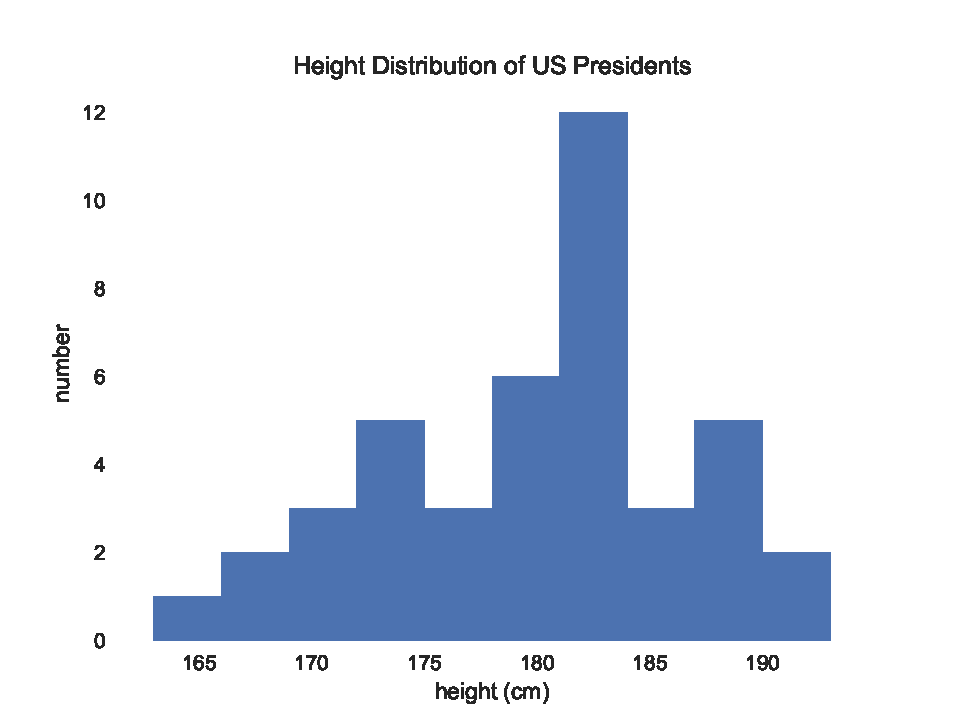
\includegraphics[width=0.4\textwidth]{figs/presidents.pdf}	
\end{frame}

\subsection{Broadcasting}
\begin{frame}[fragile]{NumPy}{Universal functions: Broadcasting (I)}
	Broadcasting is a mechanism to operate over arrays of different sizes
	\begin{itemize}
		\item Used in ufuncs
		\item Implicit array expansion through three rules
	\end{itemize}
	\vspace{-0.2cm} 
	\begin{columns}
 	   \column{0.9\textwidth}
		\begin{block}{\footnotesize{Broadcasting rules}}
		\vspace{-0.2cm} 
		\begin{enumerate}
		\item Rule 1: If the two arrays differ in their number of dimensions, the shape of the one with fewer dimensions is padded with ones on its leading (left) side.
		\item Rule 2: If the shape of the two arrays does not match in any dimension, the array with shape equal to 1 in that dimension is stretched to match the other shape.
		\item Rule 3: If in any dimension the sizes disagree and neither is equal to 1, an error is raised.
		\end{enumerate}
		\vspace{-0.2cm} 
		\end{block}
	\end{columns}
\end{frame}

\begin{frame}[fragile]{NumPy}{Universal functions: Broadcasting (II)}
	\vspace{-0.2cm} 
	\begin{columns}
 	   \column{0.7\textwidth}
		\centering 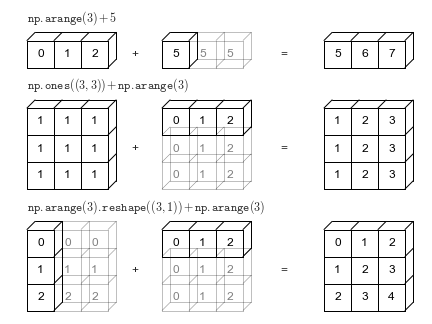
\includegraphics[width=\textwidth]{figs/02.05-broadcasting.png}	
 	   \column{0.3\textwidth}
	   	Array expansion does not consume memory!
	\end{columns}
\end{frame}

\begin{frame}[fragile]{NumPy}{Universal functions: Broadcasting (III)}
	\vspace{-0.2cm} 
	\begin{columns}
 	   \column{0.7\textwidth}
		\begin{exampleblock}{Normalization}
		\vspace{-0.2cm} 
			\begin{lstlisting}
			X = np.random.random((10, 3))
			Xmean = X.mean(0)
			X_centered = X - Xmean
			\end{lstlisting}
		\vspace{-0.2cm} 
		\end{exampleblock}

		\begin{exampleblock}{3D plot}
		\vspace{-0.2cm} 
			\begin{lstlisting}[language=Python]
			%matplotlib inline
			import matplotlib.pyplot as plt

			x = np.linspace(0, 5, 50)
			y = np.linspace(0, 5, 50)[:, np.newaxis]
			z = np.sin(x)**10+np.cos(10+y*x)*np.cos(x)

			plt.imshow(z, origin='lower', 
			    extent=[0, 5, 0, 5], cmap='viridis')
			plt.colorbar();
			\end{lstlisting}
		\vspace{-0.2cm} 
		\end{exampleblock}

 	   \column{0.3\textwidth}
			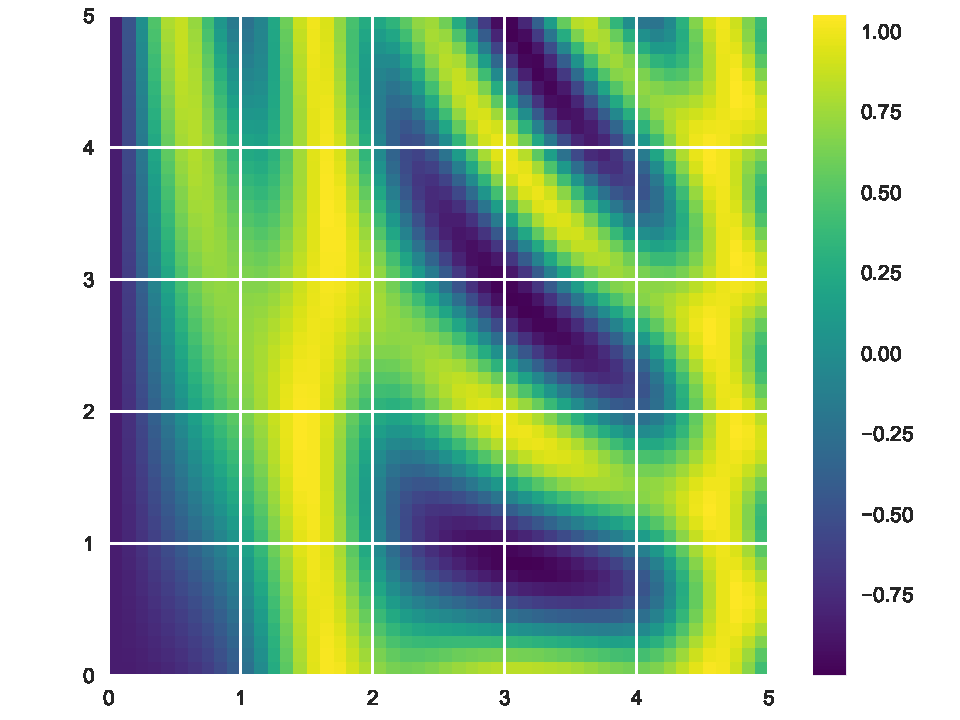
\includegraphics[width=\textwidth]{figs/3dplot.pdf}	
	\end{columns}
\end{frame}

\begin{frame}[fragile]{NumPy}{Comparisons, masks, and Boolean logic (I)}
	\vspace{-0.2cm} 
	\begin{columns}
 	   \column{0.9\textwidth}
		\href{https://raw.githubusercontent.com/jakevdp/PythonDataScienceHandbook/master/notebooks/data/Seattle2014.csv}{(Download dataset)}
		\begin{exampleblock}{Example}
		\vspace{-0.2cm} 
			\begin{lstlisting}
			import numpy as np
			import pandas as pd
             
			# pandas to extract rainfall inches as a ndarray
			rainfall = pd.read_csv('Seattle2014.csv')['PRCP'].values
			inches = rainfall / 254.0  # 1/10mm -> inches
			inches.shape 
			# Outputs (365,)
			 
			%matplotlib 
			import matplotlib.pyplot as plt
			import seaborn; seaborn.set()
			plt.hist(inches, 40);
			\end{lstlisting}
		\vspace{-0.2cm} 
		\end{exampleblock}
	\end{columns}
\end{frame}

\begin{frame}[fragile]{NumPy}{Comparisons, masks, and Boolean logic (II)}
	\begin{columns}
 	   \column{0.4\textwidth}
		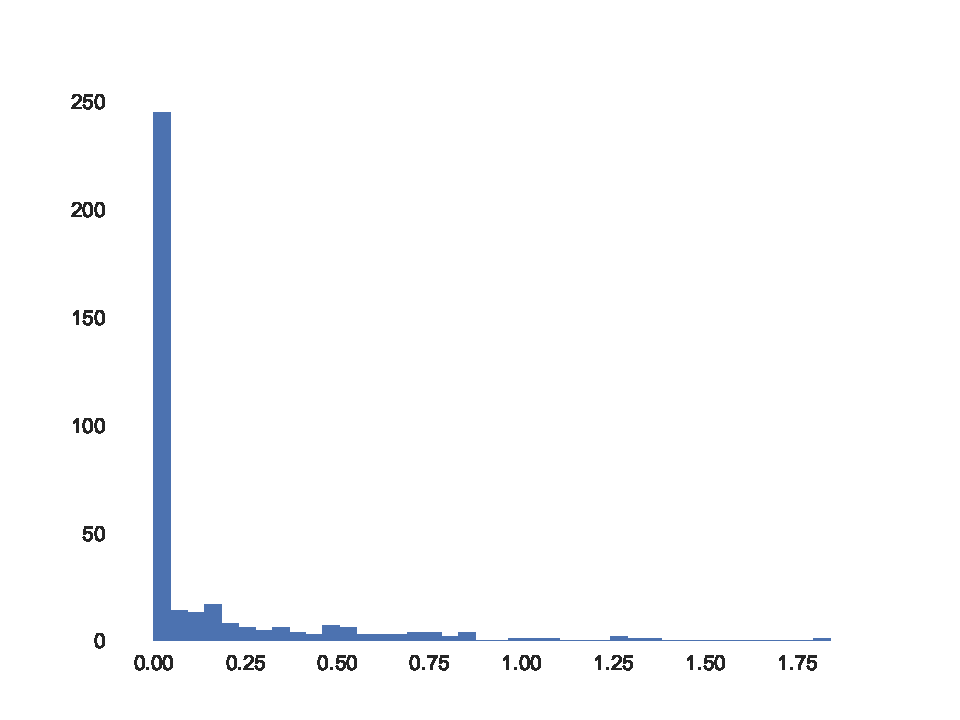
\includegraphics[width=\textwidth]{figs/rain.pdf}	
	\end{columns}

	Data filtering is a recurrent task
	\begin{itemize}
		\item How many rainy days were there in the year?
		\item What is the average precipitation on those rainy days?
		\item How many days were there with more than half an inch of rain?
	\end{itemize}

	Two filtering methods in NumPy
	\begin{itemize}
		\item Boolean arrays masks
		\item Fancy indexing
	\end{itemize}
\end{frame}

\begin{frame}[fragile]{NumPy}{Comparisons, masks, and Boolean logic: Booleans arrays masks (I)}
	
	\begin{columns}
 	   \column{0.3\textwidth}
		\begin{exampleblock}{\footnotesize{Syntax examples}}
		\vspace{-0.2cm} 
			\begin{lstlisting}
				x[x<5]
				x[x==3]
				x[(x>3)&(x<=5)]
			\end{lstlisting}
		\vspace{-0.2cm} 
		\end{exampleblock}
	\end{columns}

	\bigskip

	We've seen arithmetic ufuncs ...
	\begin{itemize}
		\item ... but they also support comparison and boolean operations
		\item Return an array of booleans
	\end{itemize}

	\footnotesize{
	\begin{columns}
 	   \column{0.5\textwidth}
       \begin{tabular}{ll}\hline
       	\textsc{Operator} &  \textsc{Ufunc}\\ \hline
       	== & \texttt{np.equal}  \\
       	!= & \texttt{np.not\_equal}  \\
       	<  & \texttt{np.less}  \\
       	<= & \texttt{np.less\_equal}  \\
       	>  & \texttt{np.greater}  \\
       	>= & \texttt{np.greater\_equal}\\\hline
    	\end{tabular}

 	   \column{0.5\textwidth}
        \begin{tabular}{ll}\hline
       	\textsc{Operator} &  \textsc{Ufunc}\\ \hline
       	\& & \texttt{np.bitwise\_and} \\
       	|  & \texttt{np.bitwise\_or}  \\
       	\textasciicircum & \texttt{np.bitwise\_xor} \\
       	\textasciitilde & \texttt{np.bitwise\_not} \\\hline
    	\end{tabular}
	\end{columns}
	}
\end{frame}

\begin{frame}[fragile]{NumPy}{Comparisons, masks, and Boolean logic: Booleans arrays masks (II)}
	
	\begin{columns}
 	   \column{0.7\textwidth}
		\begin{exampleblock}{\footnotesize{Example}}
		\vspace{-0.2cm} 
			\begin{lstlisting}
				print(x)
				[[5, 0, 3, 3]
				 [7, 9, 3, 5]
				 [2, 4, 7, 6]]
				np.count_nonzero(x < 6) # Returns 8
				np.sum(x < 6) # Returns 8
				np.sum(x < 6, axis=1) # By row, returns array([4,2,2])
				np.any(x > 8) # Returns True
				np.any(x < 0) # Returns False
				np.all(x < 10)# Returns True

				np.sum(~((inches <= 5) | (inches >= 1)))
			\end{lstlisting}
		\vspace{-0.2cm} 
		\end{exampleblock}
	\end{columns}
\end{frame}

\begin{frame}[fragile]{NumPy}{Comparisons, masks, and Boolean logic: Fancy indexing}
	\begin{columns}
 	   \column{0.4\textwidth}
	So far we've seen three accessing methods
	\begin{itemize}
		\item Simple indices (\texttt{x[1]})
		\item Slices (\texttt{x[:5]})
		\item Boolean masks (\texttt{x[x>0]})
	\end{itemize}
	Fancy indexing: Pass arrays on indices instead of scalars
 	   \column{0.6\textwidth}
		\begin{exampleblock}{\footnotesize{Example}}
		\vspace{-0.2cm} 
			\begin{lstlisting}
				x = rand.randint(100, size=10)
				[x[3], x[7], x[2]] # Simple indices
				ind = [3, 7, 4] # Array of indices
				x[ind] # Fancy indexing
				x[[3,5,6]] # Also valid
			\end{lstlisting}
		\vspace{-0.2cm} 
		\end{exampleblock}

		\footnotesize{
		\begin{alertblock}{}
		The shape of the result reflects the shape of the index arrays rather than the shape of the array being indexed
		\end{alertblock}
		}
	\end{columns}
\end{frame}

\subsection{Structured arrays}
\begin{frame}[fragile]{NumPy}{Structured arrays (I)}
	Some times, we need to group data
	\begin{itemize}
		\item Example: Store name, age and weight of several people
		\item Different data types for each attribute
	\end{itemize}
	\begin{columns}
 	   \column{\textwidth}
		\begin{exampleblock}{\footnotesize{Non-structured array}}
		\vspace{-0.2cm} 
		\begin{lstlisting}
			name = ['Alice', 'Bob', 'Cathy', 'Doug']
			age = [25, 45, 37, 19]
			weight = [55.0, 85.5, 68.0, 61.5]
		\end{lstlisting}
		\vspace{-0.2cm} 
	\end{exampleblock}
	
	\vspace{-0.2cm}
	\begin{flushleft}
	Solution: Structured arrays
	\end{flushleft}
	\vspace{-0.2cm}
	\begin{exampleblock}{\footnotesize{Structured arrays}}
		\vspace{-0.2cm} 
		\begin{lstlisting}
		# Use a compound data type for structured arrays
		data = np.zeros(4, dtype={'names':('name', 'age', 'weight'),
                          'formats':('U10', 'i4', 'f8')})
		\end{lstlisting}
		\vspace{-0.2cm} 
	\end{exampleblock}
	\end{columns}
\end{frame}

\begin{frame}[fragile]{NumPy}{Structured arrays (II)}
	\begin{columns}
 	   \column{0.6\textwidth}
	\begin{exampleblock}{\footnotesize{Structured array manipulation}}
		\vspace{-0.2cm} 
		\begin{lstlisting}
		data['name'] = name
		data['age'] = age
		data['weight'] = weight

		# Get all names
		data['name']
		# Get first row of data
		data[0]
		# Get the name from the last row
		data[-1]['name']
		# Get names where age is under 30
		data[data['age'] < 30]['name']
		\end{lstlisting}
		\vspace{-0.2cm} 
	\end{exampleblock}

	\bigskip

	\end{columns}
	These kind of structures are day-to-day used
	\begin{itemize}
		\item Pandas is a much better choice
	\end{itemize}
\end{frame}


\section{Pandas}
\subsection{Introduction}

\begin{frame}[fragile]{Pandas}{Introduction}
	\begin{columns}
 	   \column{0.6\textwidth}

	A data science workflow needs more features
	\begin{itemize}
		\item Label columns and rows
		\item Missing data
		\item Operations on groups
		\item Data input
	\end{itemize}
	Pandas implements all those features, and more
	\begin{itemize}
		\item Built on NumPy's ndarray
	\end{itemize}
	Pandas provides two main objects
	\begin{itemize}
		\item \texttt{Series}
		\item \texttt{DataFrame}
	\end{itemize}

 	   \column{0.4\textwidth}
		\begin{block}{\footnotesize{Convention}}
		\vspace{-0.2cm} 
			\begin{lstlisting}
			import numpy as np
			import pandas as pd
			\end{lstlisting}
		\vspace{-0.2cm} 
		\end{block}
	\end{columns}
\end{frame}

\subsection{The Pandas \texttt{Series} object}
\begin{frame}[fragile]{Pandas}{Introduction}
	\begin{columns}
 	   \column{0.6\textwidth}
		A DS/ML workflow needs more features
		\begin{itemize}
			\item Missing data
			\item Data input
			\item Operations on groups
			\item Label columns and rows
		\end{itemize}
		Pandas provides all those features, and more
		\begin{itemize}
			\item Pandas = \textbf{PAN}el \textbf{DA}ta \textbf{S}ystem
			\item Built on NumPy's ndarray
			\item Provides \alert{dataframes}
		\end{itemize}
		Pandas provides two main objects
		\begin{itemize}
			\item \texttt{Series} and \texttt{DataFrame}
		\end{itemize}

 	   \column{0.4\textwidth}
		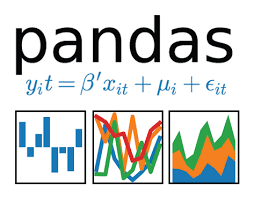
\includegraphics[width=\textwidth]{figs/pandas.png}	

		\begin{block}{\footnotesize{Convention}}
		\vspace{-0.2cm} 
			\begin{lstlisting}
			import numpy as np
			import pandas as pd
			\end{lstlisting}
		\vspace{-0.2cm} 
		\end{block}

	\end{columns}
\end{frame}

\begin{frame}[fragile]{Pandas}{The Pandas \texttt{Series} object (I)}
	\begin{columns}
 	   \column{0.6\textwidth}

		A \texttt{Series} is a one-dimensional array of indexed data
		\begin{itemize}
			\item NumPy arrays indices are implicit (i.e. its position)
			\item Series indices are explicit, and can be any type
		\end{itemize}
		Two attributes
		\begin{itemize}
			\item \texttt{values}: ndarray
			\item \texttt{index}: \texttt{pd.Index} object
		\end{itemize}
		Two indices
		\begin{itemize}
			\item Implicit: Regular index
			\item Explicit: Custom index
		\end{itemize}

 	   \column{0.4\textwidth}
	   \centering
      	\begin{tabularx}{2.7cm}{|c|c|}
			\hline
       		\textsc{Index} &  \textsc{Values}\\ \hline
       		\textit{'a'} & 0.25 \\
       		\textit{'b'} & 0.5  \\
       		\textit{'c'} & 0.75 \\
       		\textit{'d'} & 0.99 \\\hline
    	\end{tabularx}

		\bigskip

		\begin{exampleblock}{}
		\vspace{-0.2cm} 
			\begin{lstlisting}
			data = pd.Series([0.25, 0.5, 0.75, 1.0])
			data.values
			data.index
			data[1:3]
			\end{lstlisting}
		\vspace{-0.2cm} 
		\end{exampleblock}
	\end{columns}
\end{frame}

\begin{frame}[fragile]{Pandas}{The Pandas \texttt{Series} object (II)}
	\begin{columns}
 	   \column{0.8\textwidth}
		\begin{exampleblock}{\footnotesize{Custom indices}}
		\vspace{-0.2cm} 
			\begin{lstlisting}
			In[1] : data = pd.Series([0.25, 0.5, 0.75, 1.0],
			                   index=['a', 'b', 'c', 'd'])
			In [2]: data
			Out[1]: 
			a    0.25
			b    0.50
			c    0.75
			d    1.00
			dtype: float64

			In [3]: data['a']
			Out[2]: 0.25
			In [4]: data[0]
			Out[3]: 0.25
			\end{lstlisting}
		\vspace{-0.2cm} 
		\end{exampleblock}
	\end{columns}
\end{frame}

\subsection{The Pandas \texttt{DataFrame} object}
\begin{frame}{Pandas}{The Pandas \texttt{DataFrame} object (I)}
	\begin{columns}
 	   \column{0.6\textwidth}
		A \texttt{DataFrame} is a 2-D tabular data structure
		\begin{itemize}
			\item Similar to a spreadsheet
			\item Homogeneous columns
			\item Heterogeneous rows
		\end{itemize}
		Two read-only attributes, both \texttt{pd.Index}
		\begin{itemize}
			\item \texttt{index}: Rows
			\item \texttt{columns}: Columns
		\end{itemize}

 	   \column{0.4\textwidth}
		\centering 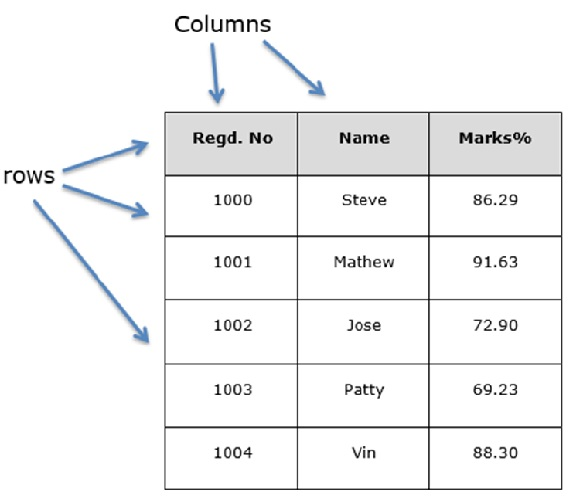
\includegraphics[width=\textwidth]{figs/structure_table.jpg}\\
		\tiny \href{https://www.tutorialspoint.com/python\_pandas/python\_pandas\_dataframe.htm}{(Source)}
	\end{columns}
\end{frame}

\begin{frame}[fragile]{Pandas}{The Pandas \texttt{DataFrame} object (II)}
	\begin{columns}
 	   \column{\textwidth}
		\begin{exampleblock}{\footnotesize{DataFrame example}}
		\vspace{-0.2cm} 
			\begin{lstlisting}
In [1]:  import seaborn as sns

In [2]:  iris = sns.load_dataset('iris')
In [3]:  iris.head()

Out[1]:
sepal_length  sepal_width  petal_length  petal_width species
0           5.1          3.5           1.4          0.2  setosa
1           4.9          3.0           1.4          0.2  setosa
2           4.7          3.2           1.3          0.2  setosa
3           4.6          3.1           1.5          0.2  setosa
4           5.0          3.6           1.4          0.2  setosa
In [246]: iris.columns
Out[246]: 
Index(['sepal_length', 'sepal_width', 'petal_length', 
        'petal_width', 'species'], dtype='object')
		\end{lstlisting}
		\vspace{-0.2cm} 
		\end{exampleblock}
	\end{columns}
\end{frame}

\subsection{Constructing \texttt{DataFrame} objects}
\begin{frame}[fragile]{Pandas}{Constructing \texttt{DataFrame} objects}
	Manual initialization
	\begin{itemize}
		\item From a single \texttt{Series} object\\
		\texttt{pd.DataFrame(population, columns=['population'])}
		\item From several \texttt{Series} objects\\
		\texttt{pd.DataFrame({'population': population,
		                       'area': area})}
		\item From a dictionary\\
	    \texttt{pd.DataFrame([\{'a': 0, 'b': 0\}, \{'a': 1, 'b': 2\}])}
		\item From a NumPy 2-D array\\
		\texttt{pd.DataFrame(np.random.rand(3, 2), \\columns=['foo', 'bar'], index=['a', 'b', 'c'])}
	\end{itemize}
	Read from a file
	\begin{itemize}
		\item CSV (very common!!!): \texttt{pd.read\_csv('filename.csv')}
		\item Excel:\\
		\texttt{pd.read\_excel('filename.xlsx', sheetname='mysheet')}
	\end{itemize}
\end{frame}

\subsection{Data indexing and selection}
\begin{frame}[fragile]{Pandas}{Data indexing and selection: \texttt{Series}}
	\begin{columns}
 	   \column{0.5\textwidth}
		\begin{exampleblock}{Dictionary-like syntax}
		\vspace{-0.2cm} 
			\begin{lstlisting}
			>>> data = pd.Series([0.25, 0.5, 0.75, 1.0], index=['a', 'b', 'c', 'd'])

			>>> 'a' in data
			True

			>>> data.keys()
			Index(['a', 'b', 'c'], dtype='object')

			>>> list(data.items())
			[('a', 0.25), ('b', 0.5), ('c', 0.75)]

			>>> data['e'] = 1.25
			\end{lstlisting}
			\vspace{-0.2cm} 
		\end{exampleblock}

		\column{0.5\textwidth}
		\begin{exampleblock}{Array-like syntax}
			\vspace{-0.2cm} 
			\begin{lstlisting}
			>> data['a':'c'] #Explicit index
			a    0.25
			b    0.50
			c    0.75
			dtype: float64
			>> data[0:2] # Implicit index
			a    0.25
			b    0.50
			dtype: float64
			>> data[data>0.5] # Masking
			c    0.75
			d    1.00
			dtype: float64
			>> data[['b','c']] # Fancy index
			b    0.50
			c    0.75
			dtype: float64
			\end{lstlisting}
			\vspace{-0.2cm} 
		\end{exampleblock}
	\end{columns}
\end{frame}

\begin{frame}[fragile]{Pandas}{Data indexing and selection: \texttt{DataFrame}}
	\begin{columns}
 	   \column{0.5\textwidth}
		\begin{exampleblock}{Dictionary-like syntax}
		\vspace{-0.2cm} 
			\begin{lstlisting}
			>>> data['area']
			>>> data.area
			>>> data.area is data['area']
			True
			>>> data['density'] = data['pop']/data['area']
			\end{lstlisting}
			\vspace{-0.2cm} 
		\end{exampleblock}

		\column{0.5\textwidth}
		\begin{exampleblock}{Array-like syntax}
		\vspace{-0.2cm} 
			\begin{lstlisting}
			>>> data.values # Get values array
			>>> data.T # Transpose
			>>> data[0] # First row
			>>> data['area'] # Area column
			\end{lstlisting}
			\vspace{-0.2cm} 
		\end{exampleblock}
	\end{columns}

	\bigskip

	Remember indexing conventions
	\begin{itemize}
		\item Indexing refers to columns (\texttt{data['area']})
		\item Slicing refers to rows (\texttt{data['Florida':'Illinois']})
		\item Masking refers to rows (\texttt{data[data.density > 100]})
	\end{itemize}
\end{frame}

\begin{frame}[fragile]{Pandas}{Data indexing and selection: loc, iloc and ix}
	\begin{columns}
 	   \column{0.5\textwidth}
	Two types of indices in Pandas
	\begin{itemize}
		\item Explicit and implicit
		\item Indexing (\texttt{data[0]}) is explit
		\item Slicing (\texttt{data[:2]}) is implicit (Python-like)
		\item Source of troubles!
	\end{itemize}
	Pandas makes explicit the used scheme
	\begin{itemize}
		\item \texttt{loc}: Explicit index
		\item \texttt{iloc}: Implicit index
		\item \texttt{ix}: Hybrid
	\end{itemize}
 	   \column{0.5\textwidth}
		\begin{exampleblock}{}
		\vspace{-0.2cm} 
			\begin{lstlisting}
			# Series
			>>> serie.loc[1]
			>>> serie.loc[1:3]
			>>> serie.iloc[1]
			>>> serie.iloc[1:3]

			# Dataframes
			>>> df.iloc[:3, :2]
			>>> df.loc[:'illinois', :'pop']
			>>> df.ix[:3, :'pop']
			>>> df.loc[df.data>100, ['pop', 'density']]
			>>> df.iloc[0, 2] = 90
			\end{lstlisting}
		\end{exampleblock}
	\end{columns}
\end{frame}

\subsection{Operating on data}

\begin{frame}[fragile]{Pandas}{Operating on data (I)}
	\begin{columns}
 	   \column{0.4\textwidth}
		Pandas fully supports NumPy's ufuncs
		\begin{itemize}
			\item Efficient computations
		\end{itemize}
		Additional Pandas features
		\begin{itemize}
			\item Index and column name preservation
			\item Index aligning
			\item Easy data combination
		\end{itemize}

 	   \column{0.6\textwidth}
		\begin{exampleblock}{}
		\vspace{-0.2cm} 
			\begin{lstlisting}
			>>> rng = np.random.RandomState(42)
			>>> df = pd.DataFrame(rng.randint(0, 10, (3,4)))
			>>> df = pd.DataFrame(rng.randint(0, 10, (3,4)), columns=['A', 'B', 'C', 'D'])
			>>> print(df)
			   A  B  C  D
			0  7  2  5  4
			1  1  7  5  1
			2  4  0  9  5
			>>> np.sin(df * np.pi / 4)
		       A       B    C    D
			 0 -7.07e-01  1.0 -0.7  1.22e-16
			 1  7.07e-01 -0.7 -0.7  7.07e-01
			 2  1.22e-16  0.0  0.7 -7.07e-01
			\end{lstlisting}
			\vspace{-0.2cm} 
		\end{exampleblock}
	\end{columns}
\end{frame}

\begin{frame}[fragile]{Pandas}{Operating on data (II)}
	\begin{columns}
 	   \column{0.8\textwidth}
		\begin{exampleblock}{Index preservation}
		\vspace{-0.2cm} 
			\begin{lstlisting}
			>>> A = pd.Series([2, 4, 6], index=[0, 1, 2])
			>>> B = pd.Series([1, 3, 5], index=[1, 2, 3])
			>>> A + B
			0    NaN
			1    5.0
			2    9.0
			3    NaN
			dtype: float64
			>>> A.add(B, fill_value=0)
			0    2.0
			1    5.0
			2    9.0
			3    5.0
			dtype: float64
			\end{lstlisting}
			\vspace{-0.2cm} 
		\end{exampleblock}
	\end{columns}
\end{frame}

\subsection{Missing data}

\begin{frame}[fragile]{Pandas}{Missing data (I)}
	NumPy supports missing data in floating-point data
	\begin{itemize}
		\item Specific value defined by IEEE
		\item Available as \texttt{np.nan}
	\end{itemize}
	Pandas supports missing data through two mechanisms
	\begin{itemize}
		\item \texttt{None} object, interpreted as NaN (\texttt{Not a Number})
		\item \texttt{np.nan}: for floating-point data
		\item Almost automatic NaN handling (types upcast)
	\end{itemize}

	\begin{columns}
 	   \column{0.55\textwidth}
		\begin{exampleblock}{}
		\vspace{-0.2cm} 
			\begin{lstlisting}
			>>> pd.Series([1, np.nan, 2, None])
			0    1.0
			1    NaN
			2    2.0
			3    NaN
			dtype: float64
			\end{lstlisting}
			\vspace{-0.2cm} 
		\end{exampleblock}
	\end{columns}
\end{frame}

\begin{frame}[fragile]{Pandas}{Missing data (II)}
	\begin{columns}
 	   \column{0.5\textwidth}
		Useful functions for missing data
		\begin{itemize}
			\item \texttt{isnull()}: Boolean mask with missing data
			\item \texttt{notnull()}: Opposite of isnull()
			\item \texttt{dropna()}: Filtered data
			\item \texttt{fillna()}: NaNs filled
		\end{itemize}

 	   \column{0.5\textwidth}
		\begin{exampleblock}{}
		\vspace{-0.2cm} 
			\begin{lstlisting}
			>>> data = pd.Series([1, np.nan, 'hello', None])
			>>> data[data.notnull()]
			0        1
			2    hello
			dtype: object

			>>> data.dropna()
			0        1
			2    hello
			dtype: object

			>>> data.fillna(0)
			0        1
			1        0
			2    hello
			3        0
			dtype: object
			\end{lstlisting}
			\vspace{-0.2cm} 
		\end{exampleblock}
	\end{columns}
\end{frame}

\subsection{Combining datasets: \texttt{pd.concat()}}

\begin{frame}[fragile]{Pandas}{Combining datasets: \texttt{pd.concat()} (I)}
	Many times we need to combine two or more datasets
	\begin{itemize}
		\item Pandas provides \texttt{pd.concat()}, \texttt{append()} and \texttt{pd.merge()}
	\end{itemize}

	\begin{columns}
    \column{0.7\textwidth}
	\begin{block}{pd.concat() signature}
	\vspace{-0.2cm} 
		\begin{lstlisting}
		pd.concat(objs, axis=0, join='outer', join_axes=None, ignore_index=False, keys=None, levels=None, names=None, verify_integrity=False, copy=True)
		\end{lstlisting}
		\vspace{-0.2cm} 
	\end{block}
	\end{columns}

	By default, \texttt{pd.concat()} joins rows preserving index
	\begin{itemize}
		\item \texttt{axis}: Join columns (\texttt{axis=1})
		\item \texttt{verify\_integrity}: Raise error if duplicates (\texttt{verify\_integrity=True})
		\item \texttt{ignore\_index}: Create new index (\texttt{ignore\_index=True})
		\item \texttt{join}: Can be 'outer' (union) or 'inner' (intersection)
	\end{itemize}
\end{frame}

\begin{frame}[fragile]{Pandas}{Combining datasets: \texttt{pd.concat()} (II)}
	\begin{columns}
 	   \column{1.1\textwidth}
		\begin{exampleblock}{}
		\vspace{-0.2cm} 
			\begin{lstlisting}
>> df1 = pd.DataFrame([{'A': 'A0', 'B': 'B0'}, {'A': 'A1', 'B': 'B1'}])
>> df2 = pd.DataFrame([{'A': 'A2', 'B': 'B2'}, {'A': 'A3', 'B': 'B3'}])

>> print(df1), print(df2); print(pd.concat([df1, df2]))
   A   B        A   B       A   B
0  A0  B0    0  A2  B2   0  A0  B0
1  A1  B1    1  A3  B3   1  A1  B1
                         0  A2  B2
                         1  A3  B3
>> pd.concat([df1, df2], axis=1)
   A   B   A   B
0  A0  B0  A2  B2
1  A1  B1  A3  B3
>> df1.append(df2)
			\end{lstlisting}
			\vspace{-0.2cm} 
		\end{exampleblock}
		\end{columns}
\end{frame}

\subsection{Combining datasets: \texttt{pd.merge()}}

\begin{frame}[fragile]{Pandas}{Combining datasets: \texttt{pd.merge()} (I)}
	Merging based on relational algebra
	\begin{itemize}
		\item Similar to databases tables joins
		\item Pretty intelligent figuring out the desired output
		\item By default, join dataframes using shared columns names
	\end{itemize}
\end{frame}

\begin{frame}[fragile]{Pandas}{Combining datasets: \texttt{pd.merge()} (II)}
	\scriptsize{
	\begin{columns}
    \column{0.45\textwidth}
		\begin{exampleblock}{One-to-one}
		\vspace{-0.2cm} 
		\begin{lstlisting}
>> print(df1); print(df2)
 employee        group
0     Bob   Accounting
1    Jake  Engineering
2    Lisa  Engineering
3     Sue           HR
 employee  hire_date
0    Lisa       2004
1     Bob       2008
2    Jake       2012
3     Sue       2014
>> print(pd.merge(df1, df2))
 employee group  hire_date
0     Bob Accounting  2008
1    Jake Engineering 2012
2    Lisa Engineering 2004
3     Sue HR          2014
		\end{lstlisting}
		\vspace{-0.2cm} 
		\end{exampleblock}

    \column{0.6\textwidth}
		\begin{exampleblock}{Many-to-one}
		\vspace{-0.2cm} 
		\begin{lstlisting}
>>> print(df3); print(df4)
  employee  group  hire_date
0      Bob   Accounting  2008
1     Jake  Engineering  2012
2     Lisa  Engineering  2004
3      Sue           HR  2014
         group  supervisor
0   Accounting  Carly
1  Engineering  Guido
2           HR  Steve
>> print(pd.merge(df3, df4))
employee  group hire_date  supervisor
0  Bob   Accounting  2008  Carly
1 Jake  Engineering  2012  Guido
2 Lisa  Engineering  2004  Guido
3  Sue           HR  2014  Steve
		\end{lstlisting}
		\vspace{-0.2cm} 
		\end{exampleblock}
	\end{columns}
	}
\end{frame}

\begin{frame}[fragile]{Pandas}{Combining datasets: \texttt{pd.merge()} (III)}
	\scriptsize{
	\begin{columns}
    \column{0.9\textwidth}
		\begin{exampleblock}{\footnotesize{Many-to-many}}
		\vspace{-0.2cm} 
		\begin{lstlisting}
>>> print(df1); print(df5)
  employee        group              group        skills
0      Bob   Accounting     0   Accounting          math
1     Jake  Engineering     1   Accounting  spreadsheets
2     Lisa  Engineering     2  Engineering        coding
3      Sue           HR     3  Engineering         linux
                            4           HR  spreadsheets
                            5           HR  organization
>>> pd.merge(df1, df5)
   employee        group        skills
0      Bob   Accounting          math
1      Bob   Accounting  spreadsheets
2     Jake  Engineering        coding
3     Jake  Engineering         linux
4     Lisa  Engineering        coding
5     Lisa  Engineering         linux
6      Sue           HR  spreadsheets
7      Sue           HR  organization
		\end{lstlisting}
		\vspace{-0.2cm} 
		\end{exampleblock}
	\end{columns}
	}
\end{frame}

\begin{frame}[fragile]{Pandas}{Combining datasets: \texttt{pd.merge()} (IV)}
	\begin{columns}
    \column{0.7\textwidth}
	\begin{block}{pd.merge() signature}
		\vspace{-0.2cm} 
		\begin{lstlisting}
		pd.merge(left, right, how='inner', on=None, left_on=None, right_on=None, left_index=False, right_index=False, sort=False, suffixes=('_x', '_y'), copy=True, indicator=False, validate=None)
		\end{lstlisting}
		\vspace{-0.2cm} 
		\end{block}
	\end{columns}
	
	\bigskip

	Arguments:
	\begin{itemize}
		\item \texttt{on}: Key column name
		\item \texttt{left\_on}: Left table key column name
		\item \texttt{right\_on}: Right table key column name
		\item \texttt{how}: Set arithmetic, \texttt{'inner'} (default, intersection), \texttt{'outer'} (union, fills missings with NaNs), \texttt{'left'} (left entries), \texttt{'right'} (right entries)
	\end{itemize}

\end{frame}

\begin{frame}[fragile]{Pandas}{Combining datasets: \texttt{pd.merge()} (V)}
	\begin{columns}
    \column{\textwidth}
	\begin{exampleblock}{}
	\vspace{-0.2cm} 
		\begin{lstlisting}
>>> A              >>> B
    lkey value         rkey value
0   foo  1         0   foo  5
1   bar  2         1   bar  6
2   baz  3         2   qux  7
3   foo  4         3   bar  8

>>> A.merge(B, left_on='lkey', right_on='rkey', how='outer')
    lkey  value_x  rkey  value_y
0   foo   1        foo   5
1   foo   4        foo   5
2   bar   2        bar   6
3   bar   2        bar   8
4   baz   3        NaN   NaN
5   NaN   NaN      qux   7
		\end{lstlisting}
		\vspace{-0.2cm} 
	\end{exampleblock}
	\end{columns}
\end{frame}

\subsection{Aggregation in Pandas}
\begin{frame}[fragile]{Pandas}{Aggregation in Pandas (I)}
	\begin{columns}
 	   \column{0.4\textwidth}
		The first step in data analysis is summarization
		\begin{itemize}
			\item First contact with data
			\item Insight to the dataset
		\end{itemize}
		Aggregation methods
		\begin{itemize}
			\item Applied to columns
		\end{itemize}
	
 	   \column{0.6\textwidth}
      	\begin{tabularx}{\textwidth}{rl}
			\hline
       		\textsc{Aggregation} &  \textsc{Description}\\ \hline
       		\texttt{count()}    & 	Total number of items \\
       		\texttt{first()}, \texttt{last()} & First and last item \\
       		\texttt{mean()}, \texttt{median()} & Mean and median \\
       		\texttt{min()}, \texttt{max()} & Minimum and maximum \\
       		\texttt{std()}, \texttt{var()} & Standard dev. and variance \\
       		\texttt{mad()} & Mean absolute deviation \\
       		\texttt{prod()} & Product of all items \\
       		\texttt{sum()} & Sum of all items \\
       		\texttt{describe()} & Data summary \\\hline
    	\end{tabularx}
	\end{columns}
\end{frame}

\begin{frame}[fragile,plain]
	\scriptsize{
	%\vspace{-0.5cm}
	\begin{columns}
 	   \column{\textwidth}
		\begin{exampleblock}{}
		\vspace{-0.2cm} 
			\begin{lstlisting}
>>> import seaborn as sns
>>> planets = sns.load_dataset('planets')
>>> planets.head()
            method number orbital_period mass distance  year
0  Radial Velocity 1      269.300        7.10    77.40  2006
1  Radial Velocity 1      874.774        2.21    56.95  2008
2  Radial Velocity 1      763.000        2.60    19.84  2011
3  Radial Velocity 1      326.030       19.40   110.62  2007
4  Radial Velocity 1      516.220       10.50   119.47  2009
>>> planets.dropna().describe()
       number  orbital_period    mass  distance      year
count  498.00      498.000000  498.00  498.0000   498.000
mean     1.73      835.778671    2.50   52.0682  2007.377
std      1.17     1469.128259    3.63   46.5960     4.167
min      1.00        1.328300    0.00    1.3500  1989.000
25%      1.00       38.272250    0.21   24.4975  2005.000
50%      1.00      357.000000    1.24   39.9400  2009.000
75%      2.00      999.600000    2.86   59.3325  2011.000
max      6.00    17337.500000   25.00  354.0000  2014.000
>>> planets.mean()
number               1.785507
orbital_period    2002.917596
mass                 2.638161
distance           264.069282
year              2009.070531
dtype: float64
			\end{lstlisting}
			\vspace{-0.2cm} 
		\end{exampleblock}
	\end{columns}
	}
\end{frame}

\subsection{Grouping in Pandas}
\begin{frame}{Pandas}{Grouping in Pandas (I)}
		Aggregation is generally used ...
		\begin{itemize}
			\item ... good to operate with the whole dataset ...
			\item ... but also is is usually insufficient
		\end{itemize}
		We need conditional aggregations
		\begin{itemize}
			\item Aggregate conditionally on some label
		\end{itemize}
		This is done with the operation \texttt{groupby} (yes, that name comes from SQL)
		\begin{itemize}
			\item Example: \texttt{df.groupby("key")}
		\end{itemize}
		Three tasks in one step
		\begin{enumerate}
			\item \textit{Split}: Break up dependening on a key
			\item \textit{Apply}: Compute some function
			\item \textit{Combine}: Merge results into an output
		\end{enumerate}
\end{frame}

\begin{frame}{Pandas}{Grouping in Pandas (II)}
	\centering 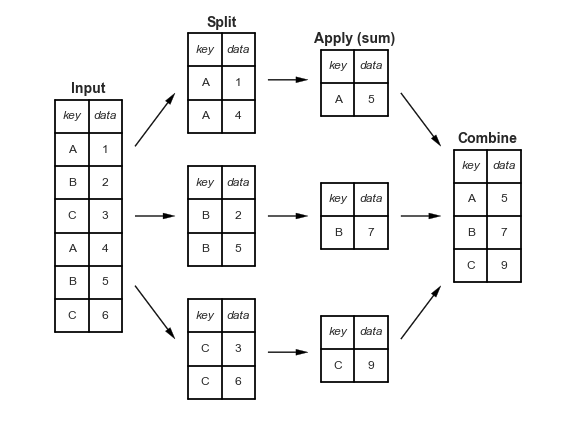
\includegraphics[width=0.9\textwidth]{figs/03.08-split-apply-combine.png}\\
\end{frame}

\begin{frame}[fragile]{Pandas}{Grouping in Pandas (III)}
	\vspace{-0.5cm}
	\begin{columns}
 	   \column{\textwidth}
		\begin{exampleblock}{}
		\vspace{-0.2cm} 
			\begin{lstlisting}
>>> df = pd.DataFrame({'key': ['A', 'B', 'C', 'A', 'B', 'C'],
                      'data': range(6)})
>>> print(df)
  key  data
0   A     0
1   B     1
2   C     2
3   A     3
4   B     4
5   C     5
>>> df.groupby('key')
<pandas.core.groupby.groupby.DataFrameGroupBy object at 0x102685438>
>>> df.groupby('key').sum()
     data
key      
A       3
B       5
C       7
			\end{lstlisting}
			\vspace{-0.2cm} 
		\end{exampleblock}
	\end{columns}
\end{frame}

\begin{frame}{Pandas}{Grouping in Pandas (III)}
	Several mapping methods available
	\begin{itemize}
		\item List\\
			  \texttt{df.groupby([2,3,4,1]).sum()}
		\item Dictionary \\
			  \texttt{df.groupby({'A': 'vowel', 'B': 'consonant', 'C': 'vowel'})}
		\item Python function \\
			  \texttt{df.groupby(str.lower)}
		\item Multiple keys \\
		      \texttt{planets.groupby(['method', 'year'])}
		\item Mixed keys \\
		      \texttt{df.groupby(['key1', 'key2', str.lower])}
	\end{itemize}
\end{frame}

\begin{frame}{Pandas}{Grouping in Pandas (IV)}
	The method \texttt{groupby()} returns an object \texttt{groupby}
	\begin{itemize}
		\item Basicly, it is a collection of dataframes\\
		      \texttt{planets.groupby('method').get\_group('Transit')}
		\item Column selection as dataframe\\
		      \texttt{planets.groupby('method')['year']}
	\end{itemize}
	Interesting groupby attribute, \texttt{groups}
	\begin{itemize}
		\item Dictionary with groups\\
		      \texttt{planets.groupby('method').groups}
		\item Compatible with the \texttt{len()} method\\
		      \texttt{len(planets.groupby('method'))}
	\end{itemize}
\end{frame}

\begin{frame}{Pandas}{Grouping in Pandas (V)}
	Usual operations with groupings
	\begin{itemize}
		\item Aggregation: \\
			\texttt{df.groupby('key').aggregate(['min', np.median, max])}\\
			\texttt{df.groupby('key').aggregate({'data1': 'min', 'data2': 'max'})}
		\item Filtering: \\
			\texttt{planets.groupby('method').filter(lambda x: x['distance'].mean() > 50.)}
		\item Transformation: \\
			\texttt{df.groupby('key').transform(lambda x: x - x.mean())}
	\end{itemize}
	Apply(): Apply arbitrary function and combine results
		\begin{itemize}
			\item Takes a function as argument that takes a DataFrame
			\item[] \texttt{planets.groupby("method").apply(lambda x: x / x.sum())}
		\end{itemize}
\end{frame}

\begin{frame}[fragile]{Pandas}{Grouping in Pandas (VI)}
	\begin{columns}
    \column{0.8\textwidth}
	\begin{exampleblock}{Grouping by decade}
	\vspace{-0.2cm} 
		\begin{lstlisting}
		decade = 10 * (planets['year'] // 10)
		decade = decade.astype(str) + 's'
		decade.name = 'decade'
		planets.groupby(['method', decade])['number'].sum().unstack().fillna(0)
		\end{lstlisting}
		\vspace{-0.2cm} 
	\end{exampleblock}
	\end{columns}
\end{frame}

\section{Visualization}
\subsection{Visualization examples}

\begin{frame}{Visualization}{Bad visualization examples (I)}
	\begin{columns}
    \column{0.5\textwidth}
		\centering 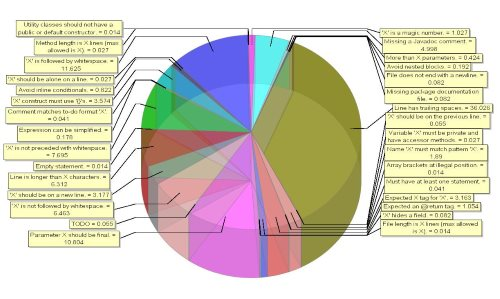
\includegraphics[width=\textwidth]{figs/bad2.jpg}\\
		\centering \tiny \href{http://livingqlikview.com/the-9-worst-data-visualizations-ever-created/}{(Source)}

    \column{0.5\textwidth}
		\centering 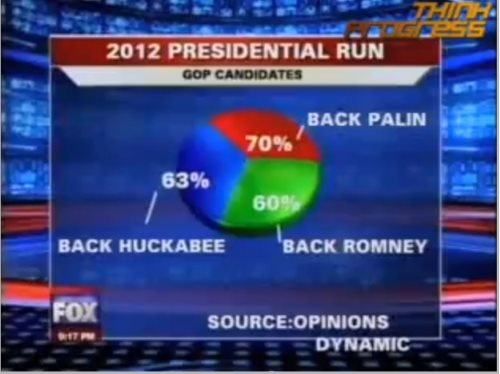
\includegraphics[width=\textwidth]{figs/bad3.jpg}\\
		\centering \tiny \href{http://livingqlikview.com/the-9-worst-data-visualizations-ever-created/}{(Source)}
	\end{columns}
\end{frame}

\begin{frame}{Visualization}{Bad visualization examples (II)}
	\begin{columns}
    \column{0.5\textwidth}
		\centering 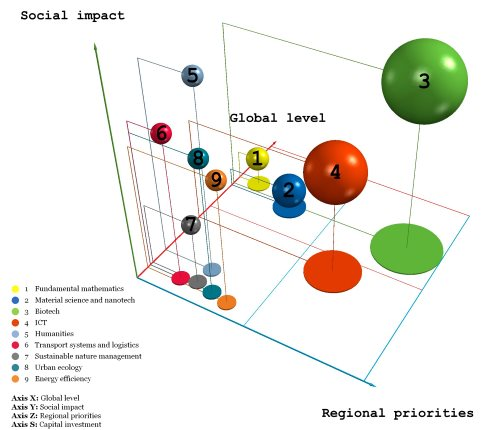
\includegraphics[width=\textwidth]{figs/bad4.jpg}\\
		\centering \tiny \href{http://livingqlikview.com/the-9-worst-data-visualizations-ever-created/}{(Source)}
    \column{0.5\textwidth}
		\centering 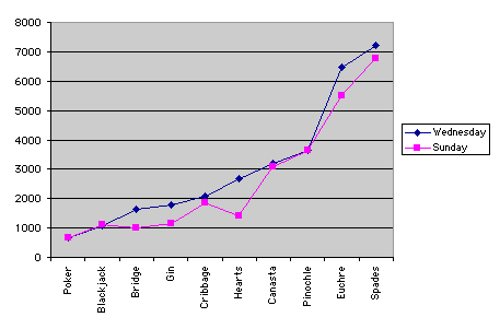
\includegraphics[width=\textwidth]{figs/bad5.jpg}\\
		\centering \tiny \href{http://livingqlikview.com/the-9-worst-data-visualizations-ever-created/}{(Source)}
	\end{columns}
\end{frame}

\begin{frame}{Visualization}{Bad visualization examples (III)}
	\begin{columns}
    \column{0.5\textwidth}
	\centering 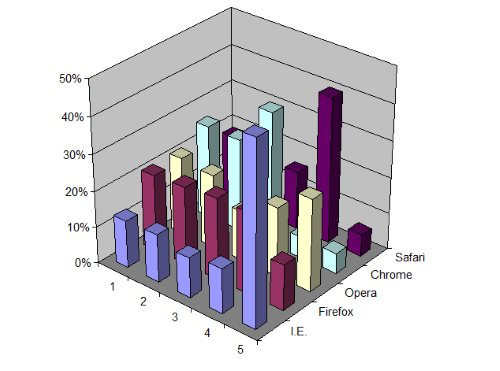
\includegraphics[width=\textwidth]{figs/bad6.jpg}\\
	\centering \tiny \href{http://livingqlikview.com/the-9-worst-data-visualizations-ever-created/}{(Source)}

    \column{0.5\textwidth}
	\centering 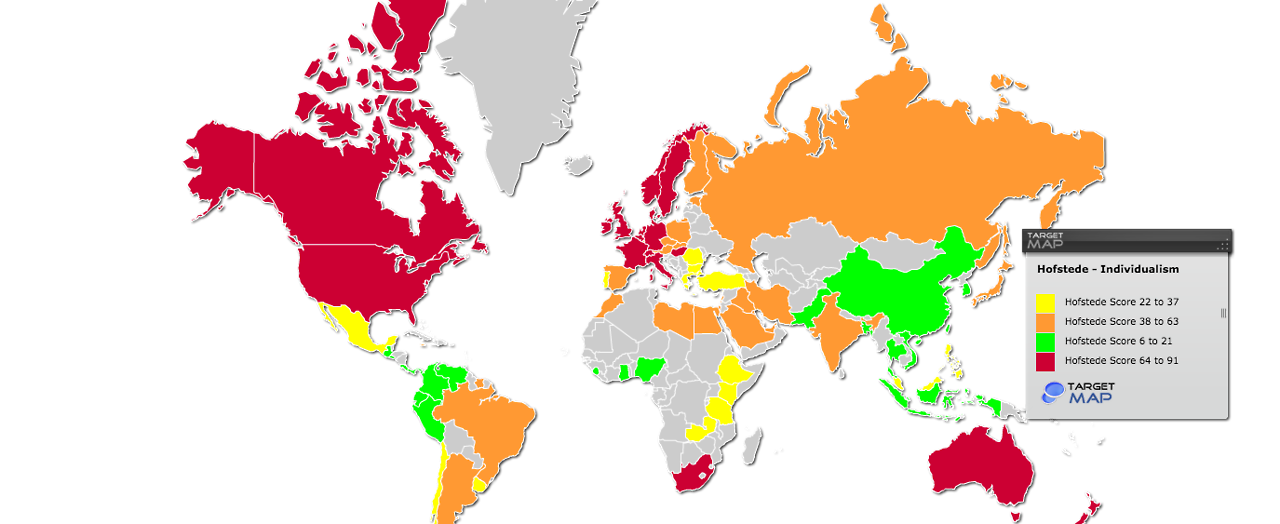
\includegraphics[width=\textwidth]{figs/bad12.png}\\
	\centering \tiny \href{http://viz.wtf/}{(Source)}
	\end{columns}
\end{frame}

\begin{frame}{Visualization}{Bad visualization examples (IV)}
	\begin{columns}
    \column{0.5\textwidth}
	\centering 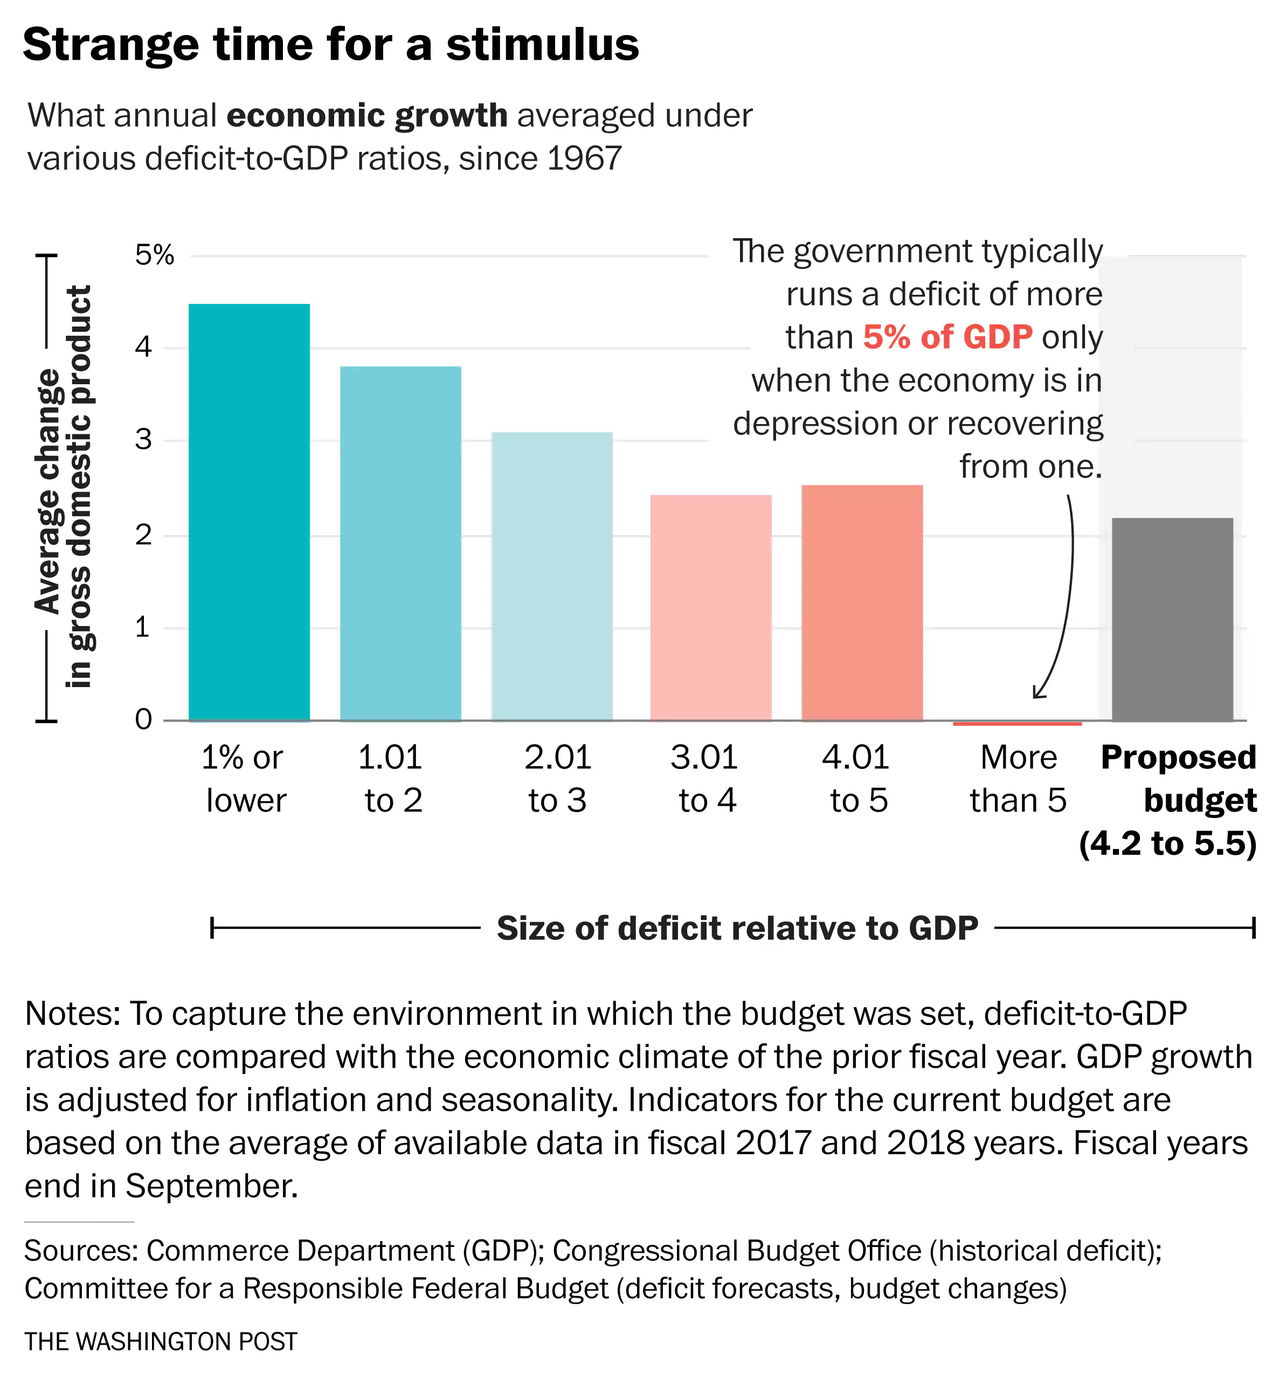
\includegraphics[width=\textwidth]{figs/bad10.png}\\
	\centering \tiny \href{http://viz.wtf/}{(Source)}

    \column{0.5\textwidth}
	\centering 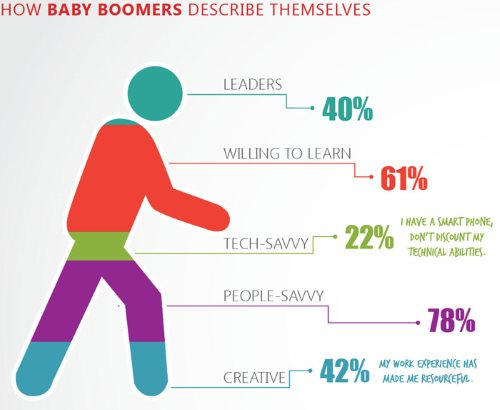
\includegraphics[width=\textwidth]{figs/bad7.jpg}\\
	\centering \tiny \href{http://livingqlikview.com/the-9-worst-data-visualizations-ever-created/}{(Source)}
	\end{columns}
\end{frame}

\begin{frame}{Visualization}{Bad visualization examples (V)}
	\begin{columns}
    \column{0.7\textwidth}
	\centering 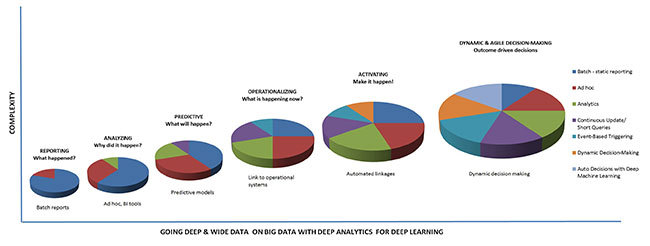
\includegraphics[width=0.8\textwidth]{figs/bad9.jpg}\\
	\centering \tiny \href{http://viz.wtf/}{(Source)}

	\bigskip

	\centering 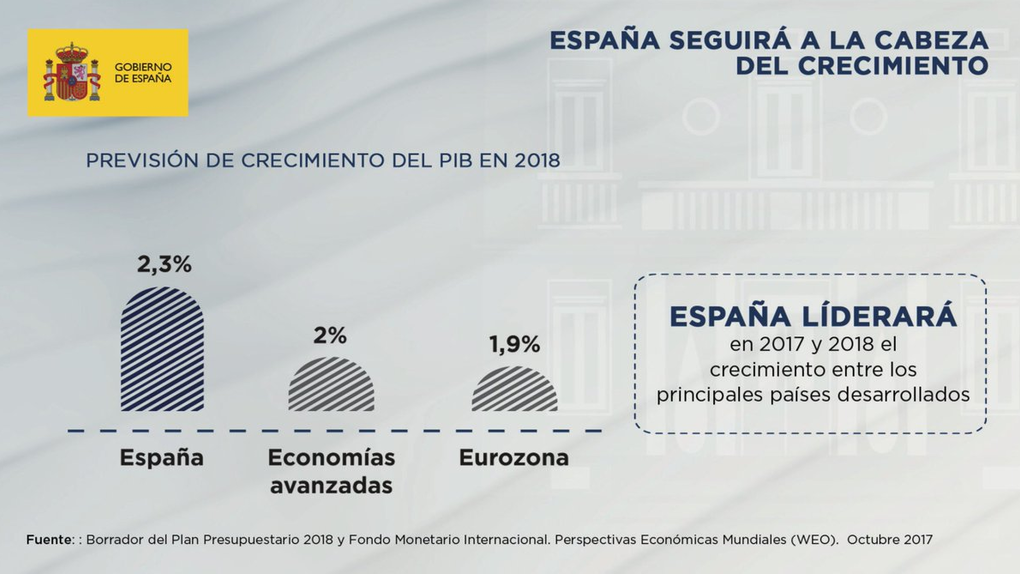
\includegraphics[width=0.8\textwidth]{figs/bad11.png}\\
	\tiny \href{http://viz.wtf/}{(Source)}
	\end{columns}
\end{frame}

\begin{frame}{Visualization}{Motivation (I)}
	Efficient data visualization tips
	\begin{itemize}
		\item \textbf{Define your story}
		\item The chart must tell the story
		\item Don't distract from your story (with irrelevant data or visual elements)
		\item One story, one chart
		\item Put the story comprension in first term
		\item Better several simple charts than one complex chart
		\item Choose colors wisely (color scale or high contrast)
		\item Elements order must support the story (leyend, bars, etc)
		\item There is life beyond pies and bars
		\item Keep it simple, stupid!
	\end{itemize}
\end{frame}

\begin{frame}{Visualization}{Motivation (II)}
	Know your data
	\begin{itemize}
		\item Categorical or numerical
		\item Number of dimensions to represent (1D, 2D, 3D, more dimensions)
	\end{itemize}
	Can you use other representation?
	\begin{itemize}
		\item Chart better than table? ...
		\item ... that depends
	\end{itemize}
	What do you want to represent?
	\begin{itemize}
		\item Distribution, relationship, comparison or composition
	\end{itemize}
	Look for templates: (\url{https://python-graph-gallery.com/})
\end{frame}

\begin{frame}[plain]{Visualization}{Motivation (III)}
	\centering 
\includegraphics[width=0.8\textwidth]{figs/chart-selection-diagram.png}\\
	\centering \tiny \href{https://flex.bi/create-beautiful-dashboard-works/}{(Source)}\\
	\href{http://experception.net/Franconeri_ExperCeptionDotNet_ChartChooser.pdf}{(Alternative resource)}
\end{frame}

\subsection{Introduction to Matplotlib}

\begin{frame}[fragile]{Visualization}{Introduction to Matplotlib (I)}
	\begin{columns}
    \column{0.5\textwidth}
	Matplotlib is a Python package
	\begin{itemize}
		\item Based on NumPy
		\item Imitates Matlab
	\end{itemize}
	Three operation modes
	\begin{itemize}
		\item Scripts. \\Must use \texttt{plt.show()} to enter event loop
		\item IPython shell. \\Must use \texttt{\%matplotlib}
		\item IPython notebool. Two modes
		\begin{itemize}
			\item \texttt{\%matplotlib inline}
			\item \texttt{\%matplotlib notebook}
		\end{itemize}
	\end{itemize}

    \column{0.5\textwidth}
	\begin{block}{\footnotesize{Convention}}
	\vspace{-0.2cm} 
	\begin{lstlisting}
	import matplotlib as mpl
	import matplotlib.pyplot as plt
	\end{lstlisting}
	\vspace{-0.2cm} 
	\end{block}

	\begin{exampleblock}{\footnotesize{myplot.py}}
	\vspace{-0.2cm} 
	\begin{lstlisting}
	import matplotlib.pyplot as plt
	import numpy as np

	x = np.linspace(0, 10, 100)

	plt.plot(x, np.sin(x))
	plt.plot(x, np.cos(x))

	plt.show()
	\end{lstlisting}
	\vspace{-0.2cm} 
	\end{exampleblock}

	\end{columns}
\end{frame}

\begin{frame}[fragile]{Visualization}{Introduction to Matplotlib (II)}
	\begin{columns}
    \column{0.5\textwidth}
	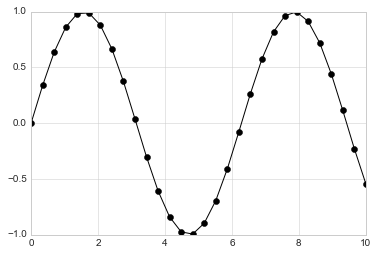
\includegraphics[width=\textwidth]{figs/matplotlib-sin.png}\\

	\begin{exampleblock}{}
	\vspace{-0.2cm} 
	\begin{lstlisting}
	plt.plot(x, np.sin(x), '-ok', color='black')
	\end{lstlisting}
	\vspace{-0.2cm} 
	\end{exampleblock}

    \column{0.5\textwidth}
	\centering 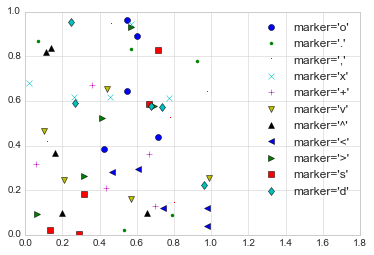
\includegraphics[width=\textwidth]{figs/matplotlib-scatterplot.png}\\
	\begin{exampleblock}{}
	\vspace{-0.2cm} 
	\begin{lstlisting}[basicstyle=\tiny]
	for marker in ['o', '.', ',', 'x', '+', 'v', '^', '<', '>', 's', 'd']:
	    plt.plot(rng.rand(5), rng.rand(5), marker,
	         label="marker='{0}'".format(marker))
	 plt.legend(numpoints=1)
	 plt.xlim(0, 1.8);
	\end{lstlisting}
	\vspace{-0.2cm} 
	\end{exampleblock}
	\end{columns}
\end{frame}

\begin{frame}[fragile]{Visualization}{Introduction to Matplotlib (III)}
	\begin{columns}
    \column{0.5\textwidth}
	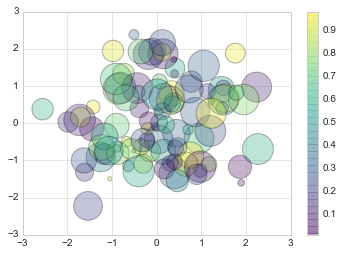
\includegraphics[width=\textwidth]{figs/matplotlib-scatterplot2.png}\\

	\begin{exampleblock}{}
	\vspace{-0.2cm} 
	\begin{lstlisting}[basicstyle=\tiny]
	rng = np.random.RandomState(0)
	x = rng.randn(100)
	y = rng.randn(100)
	colors = rng.rand(100)
	sizes = 1000 * rng.rand(100)

	plt.scatter(x, y, c=colors, s=sizes, alpha=0.3,
	            cmap='viridis')
				plt.colorbar();  # show color scale
	\end{lstlisting}
	\vspace{-0.2cm} 
	\end{exampleblock}

    \column{0.5\textwidth}
	\centering 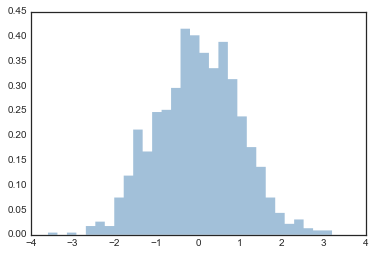
\includegraphics[width=\textwidth]{figs/matplotlib-histogram.png}\\
	\begin{exampleblock}{}
	\vspace{-0.2cm} 
	\begin{lstlisting}[basicstyle=\tiny]
	data = np.random.randn(1000)

	plt.hist(data, bins=30, normed=True, alpha=0.5,
         histtype='stepfilled', color='steelblue',
         edgecolor='none');
	\end{lstlisting}
	\vspace{-0.2cm} 
	\end{exampleblock}
	\end{columns}
\end{frame}

\begin{frame}[fragile]{Visualization}{Introduction to Matplotlib (IV)}
	\begin{columns}
    \column{0.5\textwidth}
	\begin{exampleblock}{}
	\vspace{-0.2cm} 
	\begin{lstlisting}[basicstyle=\tiny]
	ax = plt.axes(projection='3d')

	# Data for a three-dimensional line
	zline = np.linspace(0, 15, 1000)
	xline = np.sin(zline)
	yline = np.cos(zline)
	ax.plot3D(xline, yline, zline, 'gray')

	# Data for three-dimensional scattered points
	zdata = 15 * np.random.random(100)
	xdata = np.sin(zdata) + 0.1 * np.random.randn(100)
	ydata = np.cos(zdata) + 0.1 * np.random.randn(100)
	ax.scatter3D(xdata, ydata, zdata, c=zdata, cmap='Greens');
	\end{lstlisting}
	\vspace{-0.2cm} 
	\end{exampleblock}

    \column{0.5\textwidth}
	\centering 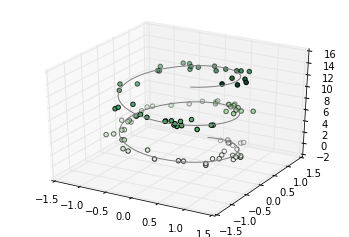
\includegraphics[width=\textwidth]{figs/matplotlib-3d.png}\\
	\end{columns}
\end{frame}

\subsection{Introduction to Seaborn}

\begin{frame}[fragile]{Visualization}{Introduction to Seaborn (I)}
	\begin{columns}
    \column{0.65\textwidth}
	Seaborn is a modern data-visualization Python package
	\begin{itemize}
		\item Based on matplotlib
		\item ... it uses matplotlib indeed
		\item Pandas-aware
		\item High level
		\item Advanced visualizations
		\item Easy to use
	\end{itemize}
	Still under development! (v. 0.9)
    \column{0.35\textwidth}
	\begin{block}{\footnotesize{Convention}}
	\vspace{-0.2cm} 
	\begin{lstlisting}
	import seaborn as sns
	\end{lstlisting}
	\vspace{-0.2cm} 
	\end{block}

	\begin{alertblock}{}
	\vspace{-0.2cm} 
	\footnotesize{This documentation is for Seaborn 0.9 or newer}
	\vspace{-0.2cm} 
	\end{alertblock}

	\end{columns}
\end{frame}

\begin{frame}[fragile]{Visualization}{Introduction to Seaborn (II)}
	\begin{columns}
    \column{0.5\textwidth}
	Display initialization
	\begin{itemize}
		\item \texttt{plt.show()}
		\item \texttt{\%matplotlib}
	\end{itemize}
	Style initialization
	\begin{itemize}
		\item Default Seaborn style \texttt{sns.set()}
		\item By default, same style than matplotlib
	\end{itemize}
	Several functions ...
	\begin{itemize}
		\item ... similar parameters
	\end{itemize}

    \column{0.5\textwidth}
	\begin{block}{Parameters}
	\begin{itemize}
		\item x: Data axis x
		\item y: Data axis Y
		\item data: Dataframe name
		\item hue: Color
		\item style: Style
		\item sizes: Size
		\item kind: Alternate representation
	\end{itemize}
	\end{block}
	\end{columns}
\end{frame}

\begin{frame}[fragile]{Visualization}{Introduction to Seaborn (III)}
	\begin{columns}
    \column{0.4\textwidth}
		\begin{block}{Typical Seaborn usage}
		\begin{enumerate}
			\item Prepare data
			\item Set up aesthetics
			\item Plot
			\item Customize the plot
		\end{enumerate}
	\end{block}


    \column{0.6\textwidth}
		\begin{exampleblock}{}
			\vspace{-0.2cm} 
			\begin{lstlisting}[basicstyle=\tiny]
			import matplotlib.pyplot as plt
			import seaborn as sns
			# Prepare data
			tips = sns.load_dataset("tips")
			# Set up aesthetics
			sns.set_style("whitegrid")
			# Plot
			g = sns.lmplot(x="tip",y="total_bill", data=tips,aspect=2)
			# Plot customization
			g = (g.set_axis_labels("Tip","Total bill(USD)").set(xlim=(0,10),ylim=(0,100)))
			plt.title("title")
			plt.show(g)
			\end{lstlisting}
			\vspace{-0.2cm} 
		\end{exampleblock}

		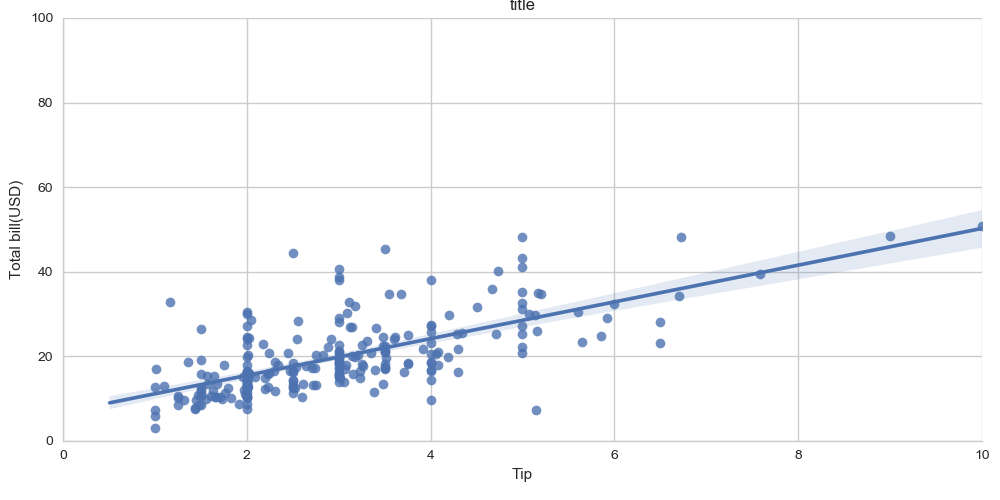
\includegraphics[width=\textwidth]{figs/sns-lm.png}\\
	\end{columns}
\end{frame}

\begin{frame}[fragile]{Visualization}{Seaborn datasets (I)}
	Seaborn comes with several dummy datasets
	\begin{itemize}
		\item \texttt{sns.load\_dataset('name')}
	\end{itemize}
	We will use two datasets
	\begin{itemize}
		\item 'iris': The classical iris dataset, numerical
		\item 'tips': Numeric and categorical variables
	\end{itemize}

	\footnotesize{
	\begin{exampleblock}{\footnotesize{Tips dataset}}
	>>> tips = sns.load\_dataset('tips')\\
	>>> print(tips.head())\\
	\begin{tabular}{lrrllllr}
		\hline
		{} &  total\_bill &   tip &     sex & smoker &  day &    time &  size \\
		\hline
		0 &       16.99 &  1.01 &  Female &     No &  Sun &  Dinner &     2 \\
		1 &       10.34 &  1.66 &    Male &     No &  Sun &  Dinner &     3 \\
		2 &       21.01 &  3.50 &    Male &     No &  Sun &  Dinner &     3 \\
		3 &       23.68 &  3.31 &    Male &     No &  Sun &  Dinner &     2 \\
		4 &       24.59 &  3.61 &  Female &     No &  Sun &  Dinner &     4 \\
		\hline
	\end{tabular}
	\end{exampleblock}
	}
\end{frame}

\begin{frame}[fragile]{Visualization}{Seaborn datasets (II)}
	\footnotesize{
	\begin{exampleblock}{\footnotesize{Iris dataset}}
	>>> iris = sns.load\_dataset('iris')\\
	>>> print(iris.head())\\
	\begin{tabular}{lrrrrl}
	\hline
	{} &  sepal\_length &  sepal\_width &  petal\_length &  petal\_width & species \\
	\hline
	0 &           5.1 &          3.5 &           1.4 &          0.2 &  setosa \\
	1 &           4.9 &          3.0 &           1.4 &          0.2 &  setosa \\
	2 &           4.7 &          3.2 &           1.3 &          0.2 &  setosa \\
	3 &           4.6 &          3.1 &           1.5 &          0.2 &  setosa \\
	4 &           5.0 &          3.6 &           1.4 &          0.2 &  setosa \\
	\hline
	\end{tabular}
	\end{exampleblock}
	}

	\centering 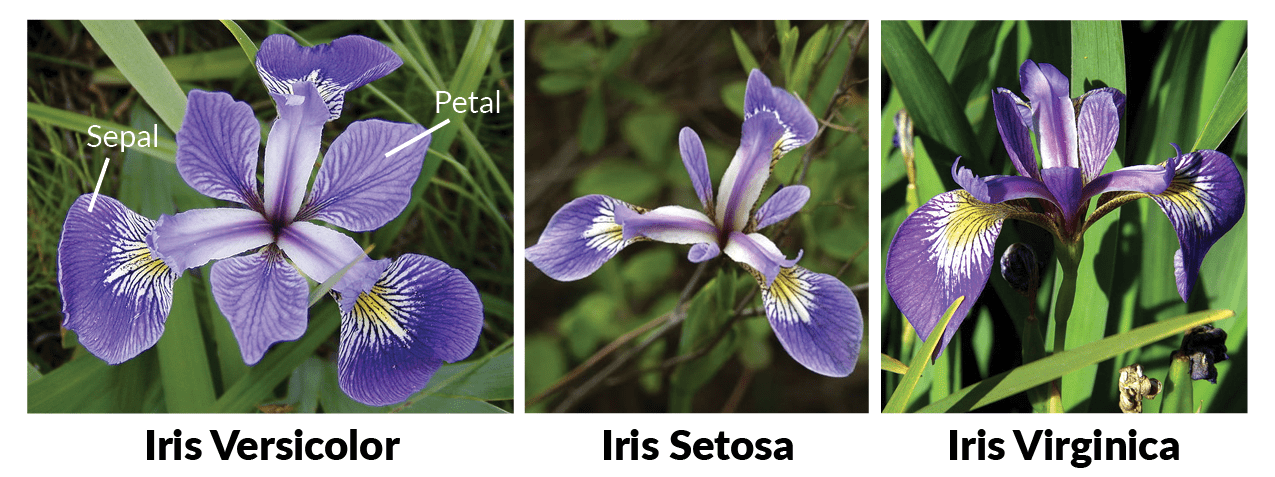
\includegraphics[width=0.7\textwidth]{figs/iris-machinelearning.png}\\
	\centering \href{http://www.lac.inpe.br/~rafael.santos/Docs/R/CAP394/WholeStory-Iris.html}{(Source)}
\end{frame}

\subsection{Seaborn: Distribution}

\begin{frame}[fragile]{Visualization}{Seaborn: Distributions (I)}
	\begin{columns}[t]
    \column{0.5\textwidth}
	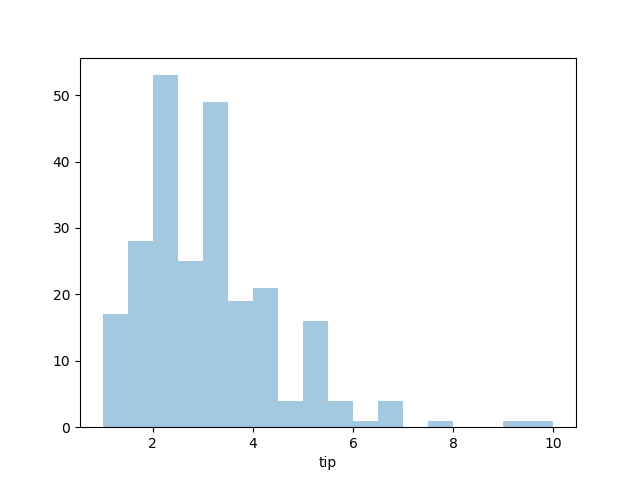
\includegraphics[width=\textwidth]{figs/sns-histogram.png}\\

	\begin{exampleblock}{\footnotesize{Histogram}}
	\vspace{-0.2cm} 
	\begin{lstlisting}[basicstyle=\small]
	sns.distplot(tips['tip'], kde=False)
	\end{lstlisting}
	\vspace{-0.2cm} 
	\end{exampleblock}

    \column{0.5\textwidth}
	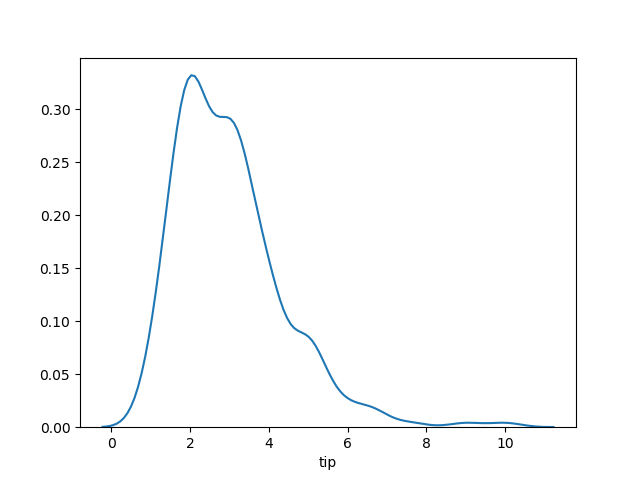
\includegraphics[width=\textwidth]{figs/sns-histogram2.png}\\
	\begin{exampleblock}{\footnotesize{Density plot}}
	\vspace{-0.2cm} 
	\begin{lstlisting}[basicstyle=\small]
	sns.distplot(tips['tip'], hist=False)
	\end{lstlisting}
	\vspace{-0.2cm} 
	\end{exampleblock}
	\end{columns}
\end{frame}

\begin{frame}[fragile]{Visualization}{Seaborn: Distributions (II)}
	\begin{columns}[t]
    \column{0.5\textwidth}
	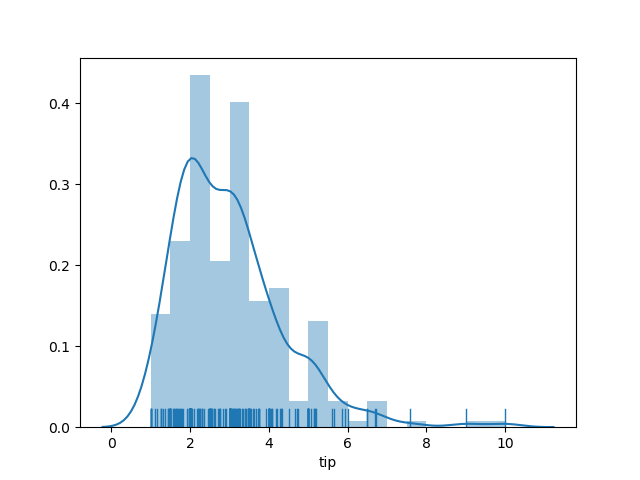
\includegraphics[width=\textwidth]{figs/sns-histogram3.png}\\

	\begin{exampleblock}{\footnotesize{Histogram + density plot}}
	\vspace{-0.2cm} 
	\begin{lstlisting}[basicstyle=\small]
	sns.distplot(tips['tip'], rug=True)
	\end{lstlisting}
	\vspace{-0.2cm} 
	\end{exampleblock}

    \column{0.5\textwidth}
	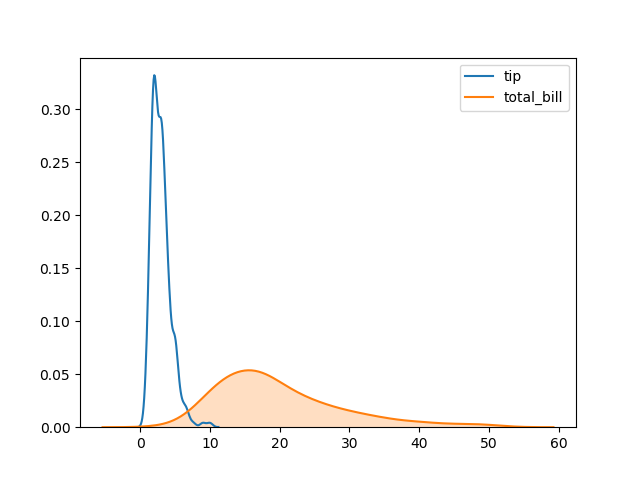
\includegraphics[width=\textwidth]{figs/sns-histogram4.png}\\
	\begin{exampleblock}{\footnotesize{Density plot}}
	\vspace{-0.2cm} 
	\begin{lstlisting}[basicstyle=\small]
	sns.kdeplot(tips['tip'])
	sns.kdeplot(tips['total_bill'], shade=True)
	\end{lstlisting}
	\vspace{-0.2cm} 
	\end{exampleblock}
	\end{columns}
\end{frame}

\begin{frame}[fragile]{Visualization}{Seaborn: Relationships (I)}
	\centering Scatterplots

	\begin{columns}[t]
    \column{0.33\textwidth}
	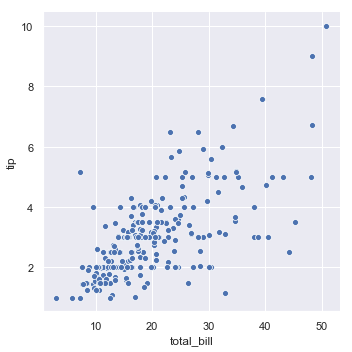
\includegraphics[width=\textwidth]{figs/sns-scatterplot.png}\\
	\begin{exampleblock}{}
	\vspace{-0.2cm} 
	\begin{lstlisting}[basicstyle=\tiny]
	sns.relplot(x="total_bill", y="tip", data=tips)
	\end{lstlisting}
	\vspace{-0.2cm} 
	\end{exampleblock}

    \column{0.33\textwidth}
	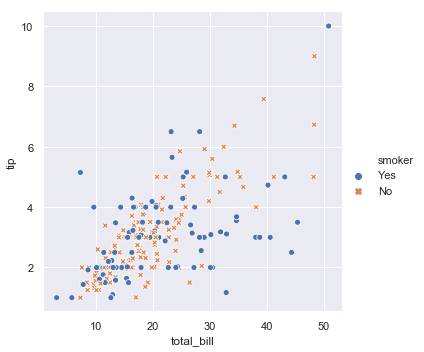
\includegraphics[width=\textwidth]{figs/sns-scatterplot2.png}\\
	\begin{exampleblock}{}
	\vspace{-0.2cm} 
	\begin{lstlisting}[basicstyle=\tiny]
	sns.relplot(x="total_bill", y="tip", hue="smoker", style="smoker", data=tips)
	\end{lstlisting}
	\vspace{-0.2cm} 
	\end{exampleblock}

    \column{0.33\textwidth}
	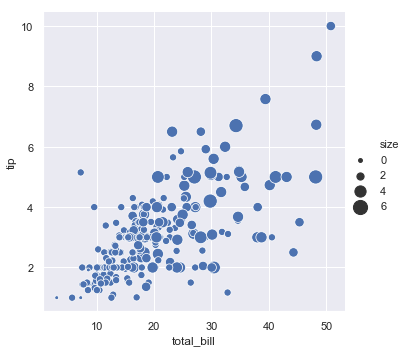
\includegraphics[width=\textwidth]{figs/sns-scatterplot3.png}\\
	\begin{exampleblock}{}
	\vspace{-0.2cm} 
	\begin{lstlisting}[basicstyle=\tiny]
	sns.relplot(x="total_bill", y="tip", size="size", sizes=(15, 200), data=tips);
	\end{lstlisting}
	\vspace{-0.2cm} 
	\end{exampleblock}

	\end{columns}

	Seaborn >= 0.9
\end{frame}

\begin{frame}[fragile]{Visualization}{Seaborn: Relationships (II)}
	\begin{columns}[t]
    \column{0.5\textwidth}
	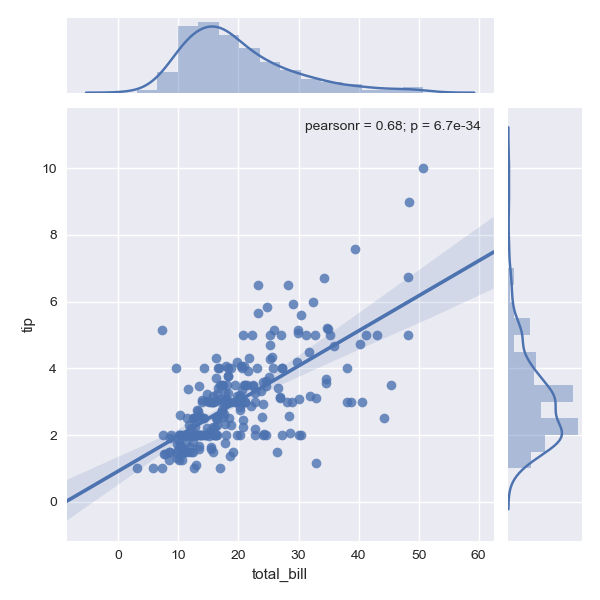
\includegraphics[width=\textwidth]{figs/sns-jointplot.png}\\
	\begin{exampleblock}{}
	\vspace{-0.2cm} 
	\begin{lstlisting}[basicstyle=\tiny]
	sns.jointplot("total_bill", "tip", tips, kind="reg")
	\end{lstlisting}
	\vspace{-0.2cm} 
	\end{exampleblock}

 	 \column{0.5\textwidth}
	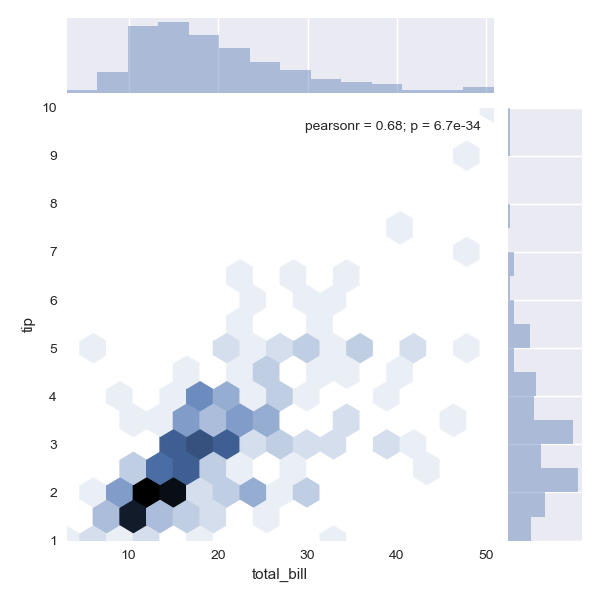
\includegraphics[width=\textwidth]{figs/sns-jointplothex.png}\\
	\begin{exampleblock}{}
	\vspace{-0.2cm} 
	\begin{lstlisting}[basicstyle=\tiny]
	sns.jointplot("total_bill", "tip", tips , kind="hex")
	\end{lstlisting}
	\vspace{-0.2cm} 
	\end{exampleblock}

	\end{columns}
\end{frame}

\begin{frame}[fragile]{Visualization}{Seaborn: Relationships (III)}
	\begin{columns}
    \column{0.5\textwidth}
	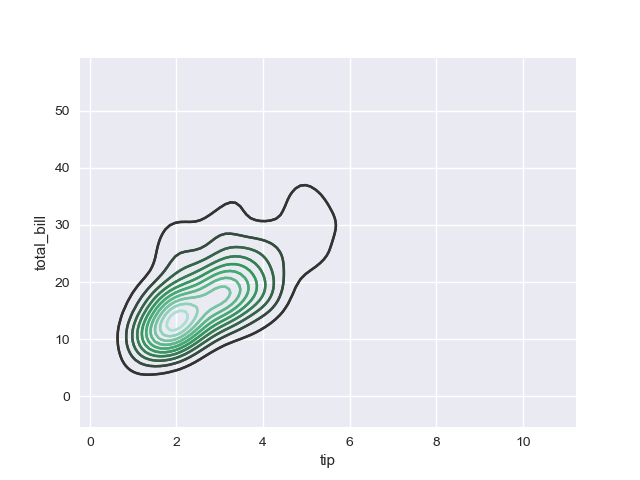
\includegraphics[width=\textwidth]{figs/sns-kdeplot.png}\\
	\begin{exampleblock}{}
	\vspace{-0.2cm} 
	\begin{lstlisting}[basicstyle=\tiny]
	sns.kdeplot(tips['tip'], tips['total_bill'])
	\end{lstlisting}
	\vspace{-0.2cm} 
	\end{exampleblock}

 	 \column{0.5\textwidth}
	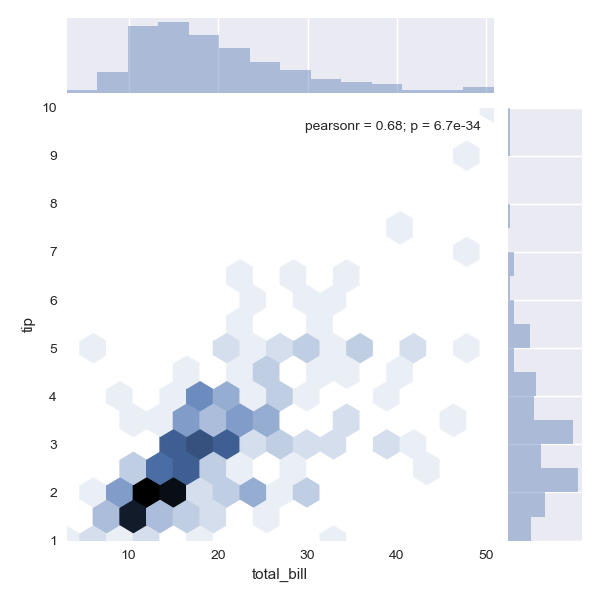
\includegraphics[width=\textwidth]{figs/sns-jointplothex.png}\\
	\begin{exampleblock}{}
	\vspace{-0.2cm} 
	\begin{lstlisting}[basicstyle=\tiny]
	sns.jointplot("total_bill", "tip", tips , kind="hex")
	\end{lstlisting}
	\vspace{-0.2cm} 
	\end{exampleblock}

	\end{columns}
\end{frame}

\begin{frame}[fragile]{Visualization}{Seaborn: Relationships (IV)}
	\begin{columns}
    \column{0.5\textwidth}
	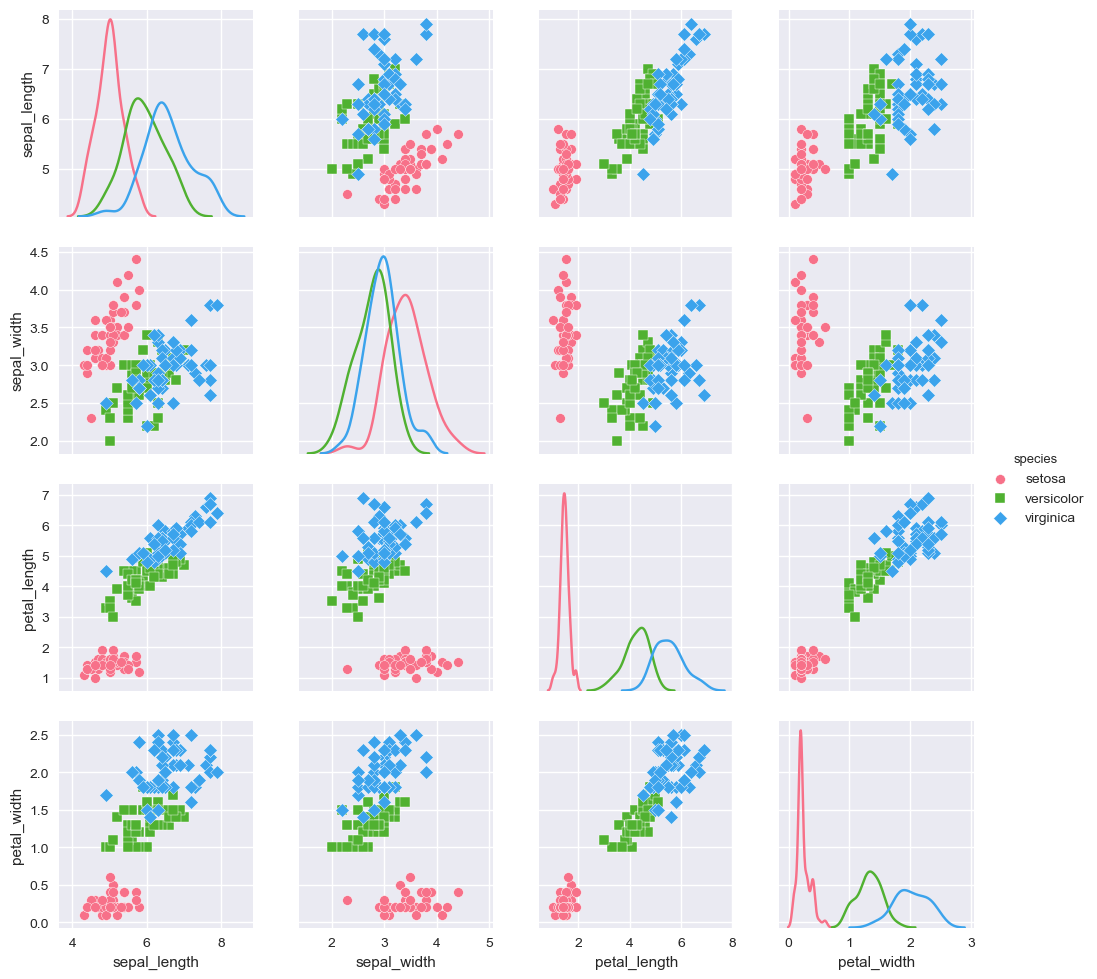
\includegraphics[width=\textwidth]{figs/sns-pairkde.png}\\
	\begin{exampleblock}{\footnotesize{Scatterplot matrix}}
	\vspace{-0.2cm} 
	\begin{lstlisting}[basicstyle=\tiny]
	sns.pairplot(iris, hue="species", palette="husl", markers=["o", "s", "D"], diag_kind='kde')
	\end{lstlisting}
	\vspace{-0.2cm} 
	\end{exampleblock}

    \column{0.5\textwidth}
	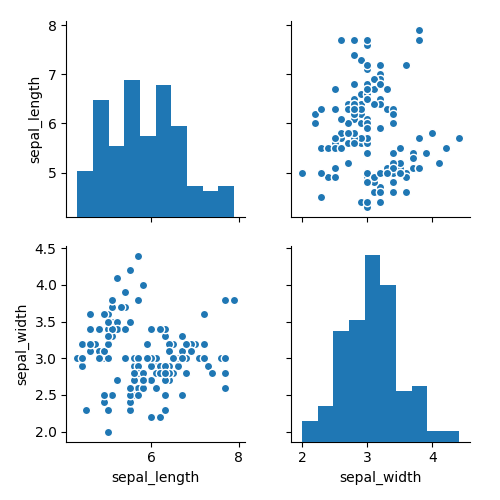
\includegraphics[width=\textwidth]{figs/sns-pair.png}\\
	\begin{exampleblock}{\footnotesize{Scatterplot matrix}}
	\vspace{-0.2cm} 
	\begin{lstlisting}[basicstyle=\tiny]
	sns.pairplot(iris, vars=["sepal_length", "sepal_width"])
	\end{lstlisting}
	\vspace{-0.2cm} 
	\end{exampleblock}

	\end{columns}
\end{frame}

\begin{frame}[fragile]{Visualization}{Seaborn: Comparisons (I)}
	\begin{columns}
    \column{0.5\textwidth}
	\includegraphics[width=\textwidth]{figs/sns-boxplot.png}\\
	\begin{exampleblock}{\footnotesize{Boxplot}}
	\vspace{-0.2cm} 
	\begin{lstlisting}[basicstyle=\tiny]
	with sns.axes_style(style='ticks'):
	    g = sns.factorplot("day", "total_bill", "sex", data=tips, kind="box")
		g.set_axis_labels("Day", "Total Bill")
	\end{lstlisting}
	\vspace{-0.2cm} 
	\end{exampleblock}

 	 \column{0.5\textwidth}
	\includegraphics[width=\textwidth]{figs/sns-violin.png}\\
	\begin{exampleblock}{\footnotesize{Violin plot}}
	\vspace{-0.2cm} 
	\begin{lstlisting}[basicstyle=\tiny]
	sns.violinplot("day", "total_bill", "sex", data=tips)
	\end{lstlisting}
	\vspace{-0.2cm} 
	\end{exampleblock}

	\end{columns}
\end{frame}

\begin{frame}[fragile]{Visualization}{Seaborn: Comparisons (II)}
	\begin{columns}
    \column{0.5\textwidth}
	\includegraphics[width=\textwidth]{figs/sns-violin2.png}\\
	\begin{exampleblock}{\footnotesize{Violin plot}}
	\vspace{-0.2cm} 
	\begin{lstlisting}[basicstyle=\tiny]
	sns.violinplot(x="day", y="total_bill", hue="sex", data=tips, split=True)
	\end{lstlisting}
	\vspace{-0.2cm} 
	\end{exampleblock}

 	 \column{0.5\textwidth}
	\centering \includegraphics[width=0.7\textwidth]{figs/violin_plots.png}\\
	\tiny \centering \href{https://xkcd.com/1967/}{(Source)}
	\end{columns}
\end{frame}

\begin{frame}[fragile]{Visualization}{Seaborn: Barplots}
	\begin{columns}
    \column{0.5\textwidth}
	\includegraphics[width=\textwidth]{figs/sns-barplot.png}\\
	\begin{exampleblock}{\footnotesize{Barplot}}
	\vspace{-0.2cm} 
	\begin{lstlisting}[basicstyle=\tiny]
	sns.barplot(x="day", y="total_bill", hue="sex", data=tips)
	\end{lstlisting}
	\vspace{-0.2cm} 
	\end{exampleblock}

    \column{0.5\textwidth}
	\includegraphics[width=\textwidth]{figs/sns-barplot2.png}\\
	\begin{exampleblock}{\footnotesize{Barplot}}
	\vspace{-0.2cm} 
	\begin{lstlisting}[basicstyle=\tiny]
	sns.barplot(x="total_bill", y="day", hue="sex", data=tips, ci=None)
	\end{lstlisting}
	\vspace{-0.2cm} 
	\end{exampleblock}
	\end{columns}
\end{frame}

\begin{frame}[fragile]{Visualization}{Seaborn: Continuity}
	\begin{columns}
    \column{0.5\textwidth}
		\includegraphics[width=0.9\textwidth]{figs/sns-line.png}\\
		\begin{exampleblock}{\footnotesize{}}
		\vspace{-0.2cm} 
		\begin{lstlisting}[basicstyle=\tiny]
		fmri = sns.load_dataset("fmri")
		sns.relplot(x="timepoint", y="signal", kind="line", data=fmri)
		\end{lstlisting}
		\vspace{-0.2cm} 
		\end{exampleblock}

 	\column{0.5\textwidth}
		\includegraphics[width=\textwidth]{figs/sns-line2.png}\\
		\begin{exampleblock}{\footnotesize{}}
		\vspace{-0.2cm} 
		\begin{lstlisting}[basicstyle=\tiny]
		sns.relplot(x="timepoint", y="signal", hue="event", kind="line", data=fmri)
		\end{lstlisting}
		\vspace{-0.2cm} 
		\end{exampleblock}
	\end{columns}
	Seaborn >= 0.9
\end{frame}

\begin{frame}[fragile]{Visualization}{Seaborn: \texttt{FacetGrid}}
	\begin{columns}
    \column{0.5\textwidth}
		\includegraphics[width=0.9\textwidth]{figs/sns-facethist.png}\\
		\begin{exampleblock}{\footnotesize{}}
		\vspace{-0.2cm} 
		\begin{lstlisting}[basicstyle=\tiny]
		fmri = sns.load_dataset("fmri")
		sns.relplot(x="timepoint", y="signal", kind="line", data=fmri)
		\end{lstlisting}
		\vspace{-0.2cm} 
		\end{exampleblock}

		Seaborn >= 0.9

 	\column{0.5\textwidth}
		\includegraphics[width=\textwidth]{figs/sns-facethist2.png}\\
		\begin{exampleblock}{\footnotesize{}}
		\vspace{-0.2cm} 
		\begin{lstlisting}[basicstyle=\tiny]
		g = sns.FacetGrid(tips, col="time", row="sex")
		g.map(sns.distplot, "tip")
		\end{lstlisting}
		\vspace{-0.2cm} 
		\end{exampleblock}
	\end{columns}
\end{frame}

\begin{frame}[plain]
	\begin{center}
		\includegraphics[width=\textwidth]{figs/self_description.png}\\
		\tiny \href{https://xkcd.com/688/}{(Source)}
	\end{center}
\end{frame}

%\begin{frame}[plain]{Solved exercise. Serializando objetos \texttt{Parcela}}{}
%	\vspace{-0.4cm}
  %  \begin{columns}
 %	   \column{0.8\textwidth}
%			\begin{block}{\footnotesize{tasaparcela\_pickle.py}}
%			\vspace{-0.2cm} 
%				\lstinputlisting[basicstyle=\ttfamily\scriptsize]{code/tasaparcela_pickle.py} % contar elementos
%			\vspace{-0.2cm} 
%			\end{block}
%	\end{columns}
	
%\end{frame}


\end{document}
